\documentclass[12pt]{report}


\usepackage[left=2.5cm, right=2.5cm, top=2.5cm, bottom=2.75cm,a4paper]{geometry}
\usepackage{booktabs,caption}
\usepackage[flushleft]{threeparttable}
\usepackage{indentfirst} %首行縮排
\usepackage[inline]{enumitem}
\usepackage{cite}

\usepackage{float}
\usepackage[section]{placeins}

\usepackage{amsmath} 
\usepackage[ruled, linesnumbered, noend, noline]{algorithm2e}

\usepackage{url}

\usepackage{graphicx} 
\usepackage{epsf}
\usepackage{amsmath}
\usepackage{comment}
\usepackage{amssymb}
\usepackage{array}
\usepackage{setspace}
\usepackage{multirow}
\usepackage{amsthm}
\usepackage{xcolor}
\usepackage{colortbl}
\theoremstyle{plain}
\newtheorem{definition}{Definition}
\newtheorem{remark}{Remark}
\usepackage{mathtools}
\usepackage{tabularx}
\usepackage{tabulary}
\usepackage{titlesec, titletoc}

\usepackage{fontspec}
\XeTeXlinebreaklocale "zh"
\XeTeXlinebreakskip = 0pt plus 1pt
\usepackage{xeCJK}
\xeCJKsetup{AutoFakeBold=true, AutoFakeSlant=true}
\usepackage{CJKnumb}
\usepackage{ragged2e} 
\usepackage[hidelinks]{hyperref}

\usepackage{subfig}
\usepackage{tikz}
\usepackage[framemethod=tikz]{mdframed}

\newtheorem{thm}{Theorem}
\newtheorem{dfn}{Definition}
\newcommand{\bdfn}{\begin{dfn}\begin{rm}}
\newcommand{\edfn}{\end{rm}\end{dfn}}
\newtheorem{prop}{Proposition}
\newtheorem{lema}{Lemma}
\newtheorem{cor}{Corollary}
\newtheorem{conj}{Conjecture}
\newtheorem{ex}{Example}

\newcommand{\Dfn}[1]{Definition~\ref{#1}}
\newcommand{\Eq}[1]{Eq.~(\ref{#1})}
\newcommand{\Eqs}[2]{Eqs.~(\ref{#1}) and (\ref{#2})}
\newcommand{\Ex}[1]{Example~(\ref{#1})}
\newcommand{\Fig}[1]{Fig.~\ref{#1}}
\newcommand{\Figs}[2]{Figs.~\ref{#1} and \ref{#2}}
\newcommand{\Lema}[1]{Lemma~\ref{#1}}
\newcommand{\Thm}[1]{Theorem~\ref{#1}}
\newcommand{\Cor}[1]{Corollary~\ref{#1}}
\newcommand{\Prop}[1]{Proposition~\ref{#1}}
\newcommand{\Chap}[1]{Chapter~\ref{#1}}
\newcommand{\Sec}[1]{Section~\ref{#1}}
\newcommand{\Tab}[1]{Table~\ref{#1}}
\newcommand{\Tabs}[2]{Tables~\ref{#1} and \ref{#2}}
\newcommand{\App}[1]{Appendix~\ref{#1}}
\newcommand{\Algo}[1]{Algorithm~\ref{#1}}

\setlength{\parindent}{2em}
\setlength\baselineskip{1em}
\setlength{\parskip}{1em}
\linespread{1.5}

\defaultCJKfontfeatures{AutoFakeBold=6,AutoFakeSlant=.4}

\titlespacing*{\chapter}{0pt}{-1em}{2em}
\titlespacing*{\section}{0pt}{0em}{-1em}
\titlespacing*{\subsection}{0pt}{0em}{-1em}

\titleformat{\chapter}[block]{\centering\fontsize{20}{30}\bfseries}{Chapter\hspace{1ex}\thechapter}{0.5em}{}

% 設定目錄中的中文章節
\titlecontents{chapter}[0em]{}{Chapter\hspace{1ex}\thecontentslabel\hspace{0.5em}}{}{\titlerule*{.}\contentspage}
\titlecontents{section}[2em]{}{\thecontentslabel\,}{}{\titlerule*{.} \contentspage}
\titlecontents{subsection}[4em]{}{\thecontentslabel\,}{}{\titlerule*{.} \contentspage}


\renewcommand{\bibname}{\textbf{Reference}}
%
\setlist[enumerate]{label=\arabic*),noitemsep,topsep=0em}
\setlist[itemize]{noitemsep,topsep=0em}

\usepackage{listings}%程式碼區塊
\newfontfamily\codefont{Andale Mono}
\newcommand{\code}[1]{$\,$\colorbox{black!15}{\codefont\selectfont #1}$\,$}
\lstset{
    commentstyle=\color{magenta},
    keywordstyle=\color{cyan},
    numberstyle=\footnotesize\codefont\selectfont,
    stringstyle=\color{teal},
    basicstyle=\footnotesize\codefont\selectfont,
    breakatwhitespace=false,         
    breaklines=true,           
    numbers=left,                    
    numbersep=8pt, 
    showstringspaces=false,
    showtabs=false,      
    frame=single,
    captionpos=b, 
    tabsize=4
}

 \usepackage{draftwatermark}
 \SetWatermarkText{
\includegraphics{fig/Taipei_Tech_Logo.png}}
 \SetWatermarkScale{0.7}
 \SetWatermarkAngle{0}

 %%% Macro to disable watermark
\makeatletter
\def\watermarkoff{\@sc@wm@stampfalse}
\makeatother

%%% Macro to enable watermark
\makeatletter
\def\watermarkon{\@sc@wm@stamptrue}
\makeatother

\makeatletter
\renewcommand\@dotsep{0}% default is 4.5
\makeatother
 % change style
\usepackage{lastpage}

\newcommand{\BibTeX}{${\mathrm{B{\scriptstyle{IB}} \! T\!_{\displaystyle E} \! X}}$}

\newcommand{\pglabel}[1]{\phantomsection\label{#1}}

\newcommand\fillpic[1]{%
  \setbox0\hbox{\includegraphics*[keepaspectratio=true,]{#1}}%
  % ^ this measures the dimensions of the graphics
  \begin{tikzpicture}[overlay,%<-allow the picture to go over the page borders
   remember picture%<-access to page anchors like page.center
   ]
  \pgfmathsetmacro{\myscale}{min(\the\paperwidth/\the\wd0,\the\paperheight/\the\ht0)}%   
  % ^ compute the scale factor as the minimum of ... to make sure the graphics does not overshoot
   \node at (current page.center){\includegraphics*[keepaspectratio=true,%
    scale=\myscale]{#1}};% <- add the graphics with the appropriate scale
    % at the center of the page.
  \end{tikzpicture}}

\newcommand{\checkresult}[1]{\thispagestyle{empty}\clearpage%
\if\relax\detokenize{#1}\relax
  \DraftwatermarkOptions{stamp=false}\textcolor{red}{\Large 在此插入審定書 (無水印)}\pglabel{pg:certificate}\clearpage\DraftwatermarkOptions{stamp=true}%
\else
    {\pglabel{pg:certificate}
    \fillpic{#1}%
    }
\clearpage%
\fi}

\newcommand{\onlyverificationletter}[2]{\makeverif{#1}{#2} \end{document}}
\newcommand{\makeverif}{}

\newcommand{\zhen}{en}
\newcommand{\isen}{en}

\newcommand{\linkurl}[2]{\href{#1}{\textcolor{blue}{#2}}}
\newcommand{\linkpg}[2]{\hyperref[#1]{\textcolor{blue}{#2}}}

\newcommand*{\minwidthbox}[2]{%
  \makebox[{\ifdim#1<\width\width\else#1\fi}]{#2}%
}
\newcommand{\centerbox}[2]{\minwidthbox{#1}{\hfill #2\hfill}}
 
\newcommand{\acktitle}{誌\hspace{1em}謝}

\newcommand{\setlang}[1]{%
\def\setlangen{en}
\def\setlangarg{#1}
\ifx \setlangen\setlangarg %
    \newcommand{\maketitlepage}{\maketitlepageen}
    \newcommand{\makecoverpage}{\makecoverpageen}
    \renewcommand{\tablename}{Table}
    \renewcommand{\figurename}{Figure}
    \renewcommand{\contentsname}{Table of Contents}
    \renewcommand{\listtablename}{List of Tables}
    \renewcommand{\listfigurename}{List of Figures}
    \renewcommand{\acktitle}{Acknowledgements}
    \renewcommand{\bibname}{Reference}
    \titleformat{\chapter}[block]{\centering\fontsize{20}{30}\bfseries}{Chapter\hspace{1ex}\thechapter}{0.5em}{}
    \titlecontents{chapter}[0em]{}{Chapter\hspace{1ex}\thecontentslabel\hspace{0.5em}}{}{\titlerule*{.}\contentspage}
\else
    \newcommand{\maketitlepage}{\maketitlepagezh}
    \newcommand{\makecoverpage}{\makecoverpagezh}
    \renewcommand{\tablename}{表}
    \renewcommand{\figurename}{圖}
    \renewcommand{\contentsname}{目\hspace{1em}錄}
    \renewcommand{\listtablename}{表目錄}
    \renewcommand{\listfigurename}{圖目錄}
    \renewcommand{\acktitle}{誌\hspace{1em}謝}
    \renewcommand{\bibname}{參考文獻}
    \titleformat{\chapter}[block]{\centering\fontsize{20}{30}\bfseries}{第\CJKnumber{\thechapter}章}{1em}{}
    \titlecontents{chapter}[0em]{}{第\CJKnumber{\thecontentslabel}章\hspace{1em}}{}{\titlerule*{.}\contentspage}
\fi\let\setlangen\relax\let\setlangarg\relax}

\newcommand{\setdegree}[1]{%
\def\setdegreeen{phd}
\def\setdegreearg{#1}
\ifx \setdegreeen\setdegreearg %
    \renewcommand{\degreezh}{博士}
    \renewcommand{\degreeen}{Doctor of Philosophy}
    \renewcommand{\articletype}{Doctoral Dissertation}
    \renewcommand{\makeverif}[2]{\DraftwatermarkOptions{stamp=false}\makeverifphd{##1}{##2}\DraftwatermarkOptions{stamp=true}}
\else
    \renewcommand{\degreezh}{碩士}
    \renewcommand{\degreeen}{Master}
    \renewcommand{\articletype}{Master Thesis}
    \renewcommand{\makeverif}[2]{\DraftwatermarkOptions{stamp=false}\makeverifmaster{##1}{##2}\DraftwatermarkOptions{stamp=true}}
\fi\let\setdegreeen\relax\let\setdegreearg\relax}

\newcommand{\titlezh}{}
\newcommand{\titleen}{}
\newcommand{\authorzh}{}
\newcommand{\authoren}{}
\newcommand{\advisorzh}{}
\newcommand{\advisoren}{}
\newcommand{\degreezh}{}
\newcommand{\degreeen}{}
\newcommand{\depzh}{}
\newcommand{\depen}{}
\newcommand{\schoolzh}{}
\newcommand{\schoolen}{}
\newcommand{\yearzh}{}
\newcommand{\yearen}{}
\newcommand{\monzh}{}
\newcommand{\monen}{}
\newcommand{\semesterzh}{}
\newcommand{\semesteren}{}
\newcommand{\articletype}{}

\newcommand{\makeTOC}{\addcontentsline{toc}{chapter}{{\contentsname}}\tableofcontents}

\newcommand{\maketitlepagezh}{%
\begin{titlepage}\pglabel{pg:titlepage}
\linespread{1.5}
    \begin{center}
    {
    {\fontsize{24}{30}\selectfont
    
\includegraphics[width=0.75\textwidth]{fig/Logo1.png}\\
        {
            {\textbf{\depzh\degreezh{}班}}\\
            {\textbf{\degreezh{}學位論文}}\\
        }
    }
    {%
    \linespread{1}
    \fontsize{18}{18}\selectfont\vspace{5em}
    }
    {\fontsize{24}{28}\selectfont
        {\setlength\baselineskip{32pt}\linespread{1}
            {\textbf{\titlezh}}\\
        }
    }
    {\fontsize{20}{28}\selectfont
        {\setlength\baselineskip{32pt}\linespread{1}
            {
            \textbf{\titleen}
            }\\
            \vfil
        }
    } 
    {\fontsize{18}{18}\selectfont\linespread{1}
            {\textbf{研究生:\authorzh}}\\[4em]
            {\textbf{指導教授:\advisorzh\hspace{1em}博士}}\\[3em]
            {\textbf{中華民國\yearzh{}年\monzh}}
    }
    }
    \end{center}
\end{titlepage}%
}

\newcommand{\makecoverpagezh}{\DraftwatermarkOptions{stamp=false}%
\begin{titlepage}\pglabel{pg:coverpage}
\linespread{1.5}
    \begin{center}
    {
    {\fontsize{24}{30}\selectfont
    
\includegraphics[width=0.75\textwidth]{fig/Logo1.png}\\
        {
            {\textbf{\depzh\degreezh{}班}}\\
            {\textbf{\degreezh{}學位論文}}\\
        }
    }
    {%
    \linespread{1}
    \fontsize{18}{18}\selectfont\vspace{5em}
    }
    {\fontsize{24}{28}\selectfont
        {\setlength\baselineskip{32pt}\linespread{1}
            {\textbf{\titlezh}}\\
        }
    }
    {\fontsize{20}{28}\selectfont
        {\setlength\baselineskip{32pt}\linespread{1}
            {
            \textbf{\titleen}
            }\\
            \vfil
        }
    } 
    {\fontsize{18}{18}\selectfont\linespread{1}
            {\textbf{研究生:\authorzh}}\\[4em]
            {\textbf{指導教授:\advisorzh\hspace{1em}博士}}\\[3em]
            {\textbf{中華民國\yearzh{}年\monzh}}
    }
    }
    \end{center}
\end{titlepage}%
\clearpage\thispagestyle{empty}\mbox{}\clearpage
\DraftwatermarkOptions{stamp=true}}

%%% EN

\newcommand{\maketitlepageen}{%
\begin{titlepage}\pglabel{pg:titlepage}
\linespread{1.5}
    % \renewcommand{\baselinestretch}{1.5}
    \begin{center}
    {
    {\fontsize{24}{30}\selectfont\setlength\baselineskip{32pt}\linespread{1}
    
\includegraphics[width=0.62\textwidth]{fig/Logo2.jpg}\\
        {
            {\textbf{\depzh\degreezh{}班}}\\%
            {\textbf{\degreezh{}學位論文}}\\%
            {\fontsize{20}{28}\selectfont\setlength\baselineskip{32pt}\linespread{1}%
            {\textbf{\depen}}\\
            % {\textbf{\degreeen{} Thesis}}\\
            {\textbf{\articletype}}\\
            }
        }
    }
    {%
    \linespread{1}
    \fontsize{18}{18}\selectfont\vfill%\vspace{5em}
    }
    {\fontsize{24}{28}\selectfont
        {\setlength\baselineskip{32pt}\linespread{1}
            {\textbf{\titlezh}}\\
        }
    }
    {\fontsize{20}{28}\selectfont
        {\setlength\baselineskip{32pt}\linespread{1}
            {
            \textbf{\titleen}
            }\\
            \vfill
        }
    } 
    {\fontsize{18}{18}\selectfont\linespread{1}
            {\textbf{研究生:\authorzh}}\\
            {\textbf{Researcher: \authoren}}\\[1em]
            {\textbf{指導教授:\advisorzh\enspace{}博士}}\\
            {\textbf{Advisor: \advisoren, Ph.D.}}\\[2em]
            {\textbf{\monen\enspace{}\yearen{}}}
    }
    }
    \end{center}
\end{titlepage}%
}

\newcommand{\makecoverpageen}{\DraftwatermarkOptions{stamp=false}%
\begin{titlepage}\pglabel{pg:coverpage}
\linespread{1.5}
    \begin{center}
    {
    {\fontsize{24}{30}\selectfont\setlength\baselineskip{32pt}\linespread{1}
    
\includegraphics[width=0.62\textwidth]{fig/Logo2.jpg}\\
        {
            {\textbf{\depzh\degreezh{}班}}\\%
            {\textbf{\degreezh{}學位論文}}\\%
            {\fontsize{20}{28}\selectfont\setlength\baselineskip{32pt}\linespread{1}%
            {\textbf{\depen}}\\
            % {\textbf{\degreeen{} Thesis}}\\
            {\textbf{\articletype}}\\
            }
        }
    }
    {%
    \linespread{1}
    \fontsize{18}{18}\selectfont\vfill%\vspace{5em}
    }
    {\fontsize{24}{28}\selectfont
        {\setlength\baselineskip{32pt}\linespread{1}
            {\textbf{\titlezh}}\\
        }
    }
    {\fontsize{20}{28}\selectfont
        {\setlength\baselineskip{32pt}\linespread{1}
            {
            \textbf{\titleen}
            }\\
            \vfill
        }
    } 
    {\fontsize{18}{18}\selectfont\linespread{1}
            {\textbf{研究生:\authorzh}}\\
            {\textbf{Researcher: \authoren}}\\[1em]
            {\textbf{指導教授:\advisorzh\enspace{}博士}}\\
            {\textbf{Advisor: \advisoren, Ph.D.}}\\[2em]
            {\textbf{\monen\enspace{}\yearen{}}}
    }
    }
    \end{center}
\end{titlepage}%
\clearpage\thispagestyle{empty}\mbox{}\clearpage
\DraftwatermarkOptions{stamp=true}}

%%%

\newcommand{\makeverifmaster}[2]{\begin{titlepage}
\begin{center}
\linespread{1.2}
\fontsize{20}{22}\selectfont\bfseries
\mbox{}\\
    國立臺北科技大學\\
    研究所碩士學位論文口試委員會審定書
\end{center}

\linespread{1.8}
\fontsize{14}{14}\selectfont
\hspace{2em}本校\underline{\centerbox{6em}{\enspace#1\enspace}}研究所\underline{\centerbox{8em}{\enspace#2\enspace}}君\\[1em]
所提論文,經本委員會審定通過,合於碩士資格,特此證明。

\noindent 學位考試委員會\\
\begin{tabular}{>{\raggedleft\arraybackslash}p{5.5em}rp{10em}}
     &委\hspace{2em}員:&  \\ \cline{3-3}
     & & \\
     & & \\ \cline{3-3}
     & & \\
     & & \\ \cline{3-3}
     & & \\
     & & \\ \cline{3-3}
     & & \\
     & & \\ \cline{3-3}
     & & \\
     & & \\ \cline{3-3}
     & & \\
     & 指導教授:\\ \cline{3-3}
     & & \\
     & 所\hspace{2em}長:\\ \cline{3-3}
\end{tabular}
\vfill
\begin{center}
\fontsize{16}{16}\selectfont
中\,華\,民\,國\hspace{1em}\yearzh\hspace{1em}年\hspace{3em}月\hspace{3em}日
\end{center}
\vspace{3em}
\end{titlepage}}

\newcommand{\makeverifphd}[2]{\begin{titlepage}
\begin{center}
\linespread{1.2}
\fontsize{20}{22}\selectfont\bfseries
\mbox{}\\
    國立臺北科技大學\\
    研究所博士學位論文口試委員會審定書
\end{center}

\linespread{1.8}
\fontsize{14}{14}\selectfont
\hspace{2em}本校\underline{\centerbox{6em}{\enspace#1\enspace}}研究所\underline{\centerbox{8em}{\enspace#2\enspace}}君\\[1em]
所提論文,經本委員會審定通過,合於博士資格,特此證明。

\noindent 學位考試委員會\\
\begin{tabular}{>{\raggedleft\arraybackslash}p{5.5em}rp{10em}}
     &委員兼召集人:&  \\ \cline{3-3}
     & & \\
     &委\hspace{2em}員:& \\ \cline{3-3}
     & & \\
     & & \\ \cline{3-3}
     & & \\
     & & \\ \cline{3-3}
     & & \\
     & & \\ \cline{3-3}
     & & \\
     & & \\ \cline{3-3}
     & & \\
     & 指導教授:\\ \cline{3-3}
     & & \\
     & 所\hspace{2em}長:\\ \cline{3-3}
\end{tabular}
\vfill
\begin{center}
\fontsize{16}{16}\selectfont
中\,華\,民\,國\hspace{1em}\yearzh\hspace{1em}年\hspace{3em}月\hspace{3em}日
\end{center}
\vspace{3em}
\end{titlepage}}

\newcommand{\makecontentlists}{%目錄
\makeTOC
\newpage

%表目錄
\addcontentsline{toc}{chapter}{{\listtablename}}
\renewcommand{\numberline}[1]{{\tablename}~#1\hspace*{0.5em}}
\listoftables
\clearpage

%圖目錄
\addcontentsline{toc}{chapter}{{\listfigurename}}
\renewcommand{\numberline}[1]{{\figurename}~#1\hspace*{0.5em}} 
\listoffigures
\newpage}

\newcommand{\starttext}{\pagenumbering{arabic}\setcounter{page}{1}}

\newcommand{\showcmd}[1]{\textbackslash{}#1}

\newenvironment{init}
{%
\pagenumbering{roman}
\setcounter{page}{1}\par}
{\clearpage\pagenumbering{arabic}}

\newenvironment{abszh}[1]
{\pglabel{pg:abszh}
{\centering\fontsize{12}{12}\selectfont\linespread{1.5}\vspace{1em}
\chapter*{摘\hspace{1em}要}
\addcontentsline{toc}{chapter}{{摘\hspace{1em}要}}
\vspace{1ex}}
{\setlength\parindent{0em}
關鍵詞:{#1} \par
}
\setlength\parindent{2em}
}
{\clearpage}

\newenvironment{absen}[1]
{
{\centering\fontsize{12}{12}\selectfont\linespread{1.5}\vspace{1em}
\chapter*{ABSTRACT}
\addcontentsline{toc}{chapter}{{ABSTRACT}}
\vspace{1ex}}
{\setlength\parindent{0em}
Keyword    :{#1} \par
}
\setlength\parindent{2em}
}
{\clearpage}

\newenvironment{ack}
{
{\centering\fontsize{12}{12}\selectfont\linespread{1.5}\vspace{1em}
\chapter*{\acktitle}
\addcontentsline{toc}{chapter}{{\acktitle}}
\vspace{1ex}}
\setlength\parindent{2em}
}
{\clearpage}   % define environment and parameters
\setlang{zh}  % change the base-lang `zh`-中文 `en`-英文
\setdegree{ms} % change format of degree `ms`-碩士論文 `phd`-博士論文  

\setmainfont{Times New Roman}  % 可自定義英文內文主要字體 (預設)
\setCJKmainfont{標楷體}         % 可自定義中文內文主要字體 (Windows 內建楷體)
% \setCJKmainfont{標楷體-繁}      % 可自定義中文內文主要字體 (Mac OS 內建楷體)
% \setCJKmainfont{教育部標準楷書}  % 可自定義中文內文主要字體 (教育部提供下載的楷體)
% \setCJKmainfont{cwTeXKai}      % Overleaf 可用中文楷體
% \setCJKmainfont{TW-Kai}        % Overleaf 可用中文楷體

% Define parameters for initialization
\renewcommand{\titlezh}{集成自動化工具的 \LaTeX{} 臺北科技大學學位論文模板與使用指引}
\renewcommand{\titleen}{A User Guide for the \LaTeX Thesis Template of NTUT with Integrated Automation Tools}
\renewcommand{\authorzh}{佚名}
\renewcommand{\authoren}{Anonymous}
\renewcommand{\advisorzh}{佚名}
\renewcommand{\advisoren}{Guidonymous}
\renewcommand{\depzh}{電子工程系}
\renewcommand{\depen}{Department of Electronic Engineering}
\renewcommand{\schoolzh}{國立臺北科技大學}
\renewcommand{\schoolen}{National Taipei University of Technology}
\renewcommand{\yearzh}{一百一十四}
\renewcommand{\yearen}{2025}
\renewcommand{\monzh}{六月}
\renewcommand{\monen}{June}
\renewcommand{\semesterzh}{二}
\renewcommand{\semesteren}{2}

% \setcounter{tocdepth}{1} % 修改目錄深度

\begin{document}

%封面
\makecoverpage % 生成論文紙本封面 (僅紙本論文需要)

\maketitlepage % 生成電子論文封面 (電子論文從此頁開始)

\checkresult{} % {}中填入審定書檔名 (相對路徑上的檔名)
% \makeverif{\depzh}{\authorzh}              % 生成審定書模板,兩個參數為 {系所名}{學生名}
% \onlyverificationletter{\depzh}{\authorzh} % 生成審定書模板並終止編譯

\begin{init} % 羅馬數字標記區域

\begin{abszh}{關鍵詞1、關鍵詞2、關鍵詞3}
這是一份台北科技大學的\LaTeX{}學位論文模板,同時也是「如何用\LaTeX{}優雅地折磨自己」的入門指南。本文不僅教你如何使用模板的核心功能、調整排版,還貼心地為你準備了初學者的「踩坑大全」和「細節魔鬼」。當然,別忘了參考學校那些藏在角落裡的神祕PDF文件,以及IEEE的參考文獻格式──畢竟,誰不想在寫論文時順便成為格式大師呢?總之,這是一份讓你從\LaTeX{}小白變成「勉強能用」的必備寶典,祝你好運! --- 由 AI 總結
\end{abszh}

%英文摘要
\begin{absen}{keyword1, keyword2, keyword3,}
This is a \LaTeX{} thesis template for Taipei Tech, and it’s also a beginner-friendly guide to using \LaTeX{}. It explains the main features of the template, how to change the layout, and gives tips for common problems beginners face. You’ll also find links to helpful files from the school and learn how to format references like a pro (thanks to IEEE rules). Think of it as your cheat sheet to go from "What is \LaTeX{}?" to "I can do this!" Good luck, and have fun! ---~Summarized by AI
\end{absen}

%誌謝
\begin{ack}
首先,感謝我的指導教授,您的耐心與智慧讓我明白,研究不僅是一場與知識的搏鬥,更是一場與自己的耐力賽。感謝實驗室的同學們,你們的陪伴讓我在無數個熬夜的日子裡,零食和冷笑話一樣不可或缺。感謝我的家人和朋友,你們的支持讓我明白,即使我經常把“論文快寫完了”變成“快了快了”。

感謝所有在這段旅程中給予我幫助的人,無論是精神上的支持還是默默忍受我的抱怨。這段經歷讓我學會了如何在壓力下保持微笑(即使是在崩潰邊緣)。

終於,這篇論文不僅是學術上的成就,更是我人生中的一次重要成長與蛻變。願所有研究生都能順利畢業,迎接更美好的明天——因為我們都知道,這只是開始,而不是結束。 --- 由 AI 產生
\end{ack}

% 建立目錄
\makecontentlists

\end{init}

\chapter{Introduction}

本文是一份臺北科技大學碩博士學位論文的\LaTeX{}排版範本,同時也是本範本的引導文件與簡易的\LaTeX{}教程,在今年 (2025年) 已有使用此模板的文章通過了學校圖書館的審核。在這份教程中會
\begin{enumerate*}
    \item 簡易的介紹本範本中所提供的核心自動化功能、
    \item 本範本中的檔案結構、
    \item 如何根據自身需求調整部分排版、
    \item 初學以\LaTeX{}撰寫學位論文中常遇到的問題以及
    \item 一些可能需要額外注意的細節考量。
\end{enumerate*}
本範本的編纂過程中參考了多項文件,其中包含:
\begin{itemize}
    \item 本校(\schoolzh)法規一覽表頁面 \cite{ntutrule} 中編號為\textbf{J1}的\linkurl{https://oaa.ntut.edu.tw/var/file/8/1008/img/2966/J1.pdf}{論文撰寫規範書}與編號為\textbf{J2}的\linkurl{https://oaa.ntut.edu.tw/var/file/8/1008/img/2966/J2.pdf}{論文撰寫範例}。
    \item 本校圖書館所提供的學位論文相關說明下載區\cite{ntutlibdown},該網頁中提供了多項與學位論文有關的檔案下載。其中``學位論文編輯''表格中的\textbf{本校學位論文格式範本}。該範本中包含兩份可供參考的PDF文件於\linkurl{https://ndltdcc.ncl.edu.tw/userfiles/TIT00/files/Thesis_Template(chi)(3).pdf}{{PDF}}與\linkurl{https://ndltdcc.ncl.edu.tw/userfiles/TIT00/files/論文範本_說明版(中)(1).pdf}{{說明}}。此外,該表格中也提供了另外的\LaTeX 範本由學生分享於 \linkurl{https://github.com/ntut-xuan/NTUT-Thesis-Template}{Github}。
    \item 由於學校並無特別規定參考文獻格式,參考文獻格式應遵循各科系主流格式即可。因此,我們在參考文獻格式方面的相關說明則參考於IEEE相關規範,其中主要包含了 IEEE Reference Guide \cite{ieeerefguide} 與 How to Use the IEEEtran BibTeX Style \cite{ieeebib}這兩份文件。同時,我們也會藉由BibTeX 官方的説明 \cite{bibtex},討論如何在不使用\code{IEEEtran.bst} (IEEE提供的參考文獻風格文件) 的情況下實現IEEE的Reference格式\footnote{現在的Overleaf已經默認裝載了\code{IEEEtran.sty}與\code{IEEEtran.bst}這兩個風格化文件,可以在不依賴外部檔案的情況下直接撰寫IEEE格式的論文。若需要在本地端使用該格式則需要至\linkurl{https://ctan.org/tex-archive/macros/latex/contrib/IEEEtran/bibtex}{{CTAN}}之類的網站下載模板檔案。}
\end{itemize}
在撰寫論文的同時記得在各自系上網頁查看必要要求,並可於 \cite{ntutsheet} 查詢相關文獻以及在\cite{ntutlibcommit}確認畢業流程。另一方面,務必\textbf{注意},您的論文頁數與引用數量都應比這篇模板/介紹之內容要多得多。如果內容量不及本篇文章,請務必再擴充文本與內容。

\section{模板使用引導}

相較於更為人所知且普遍被使用的 Microsoft (MS) Word 而言,\LaTeX{}最大的優勢莫過於是
\begin{enumerate*}
    \item 更好看且方便的數學字體、
    \item 更整齊且美觀的整體文字排版以及關鍵的
    \item 排版功能的自動化和
    \item 內容與排版解耦\footnote{文字內容本身不影響排版,排版由代碼指令產生,這杜絕了一般集成GUI介面的字排版軟體 (如 MS Word) 在一部分文字內容產生變化時可能會影響其他內容排版結果的問題。}。
\end{enumerate*}
這其中``排版功能的自動化''尤為重要,這是一部分人始終使用\LaTeX{}作為文章撰寫工具的核心原因,特別是相當依賴於使用交叉引用的學術文章尤其如此。

當然,其寫作使用純文字(代碼)使(文章)內容與排版解耦合的特性使得\LaTeX{}更容易被主流的版本控制工具(Git/Github)檢索與比對、在資料壓縮過程中可以獲得更好的壓縮率,同時也更容易與其他常見格式(如: Markdown與HTML)之間相互轉換。這些也是重要的優勢,但是並不會直接的帶來體驗升級,也很難作為無可替代的原因。

對於大多數初學\LaTeX 的使用者而言,通常最先會被\code{\textbackslash{}section}指令與\textbf{數學環境}所吸引。這兩者也確實對應了\LaTeX{}最直觀的兩項功能
\begin{enumerate*}
    \item 自動編號與
    \item 可編程的複雜數學排版。
\end{enumerate*}
接下來,真正開始作業後,\code{figure}環境與\code{table}環境加入為手邊常用的工具。而\code{\textbackslash{}ref}和\code{\textbackslash{}cite}這倆引用工具的開始被使用後,``自動化''在\LaTeX{}中的涵義才真正得到體現。然而\LaTeX{}雖然是圖靈完備的程式語言,然而其語法晦澀且抽象方式相當小眾且古老,一般使用者並不會為了用其編寫自動化的排版代碼而來。反之,用戶則是為了那些已經準備好的、開箱即用的工具而來。

如今大多數可見的學位論文模板廣泛的使用\code{\textbackslash{}input}指令並將其視為``便於模組化''的開發工具。這可以讓主文件看起來簡潔,但是反而容易喪失了整合開發環境(integrated development environment, IDE)提供自動補全的便利性,也反而更難構造各個文章段落和交叉引用之間的關係。同時,在``正文之外''很多因為各人之間複用性高而真正需要模板化的部分卻沒有真正的模板化,反而需要各人手動調整。這不僅帶來了不便,而且也喪失了\LaTeX 自動化排版的巨大優勢。

在這個模板中我們不僅提供了已經經比對誤差足夠小的排版模板,同時我們也提供了自動化工具以在給定了各個研究生必須的個人訊息後可以藉由足夠直覺的指令自動生成下面頁面而無須手動修改文本與計算頁數:
\begin{enumerate}
    \item 論文封面\footnote{只有紙本需要,其排版與書名頁一致,但無須浮水印。}
    \item 空白頁
    \item 書名頁\footnote{電子論文由此開始} (有浮水印)
    \item 學位論文口試委員會審定書 (碩士、博士) (無浮水印)
    \item 中文摘要 (以下皆需要有浮水印)
    \item 英文摘要
    \item 誌謝
    \item 目錄
    \item 表目錄
    \item 圖目錄
    \item 正文
    \item 參考文獻
\end{enumerate}
除此之外,針對誌謝、目錄、表目錄、圖目錄、參考文獻與章節標題格式這些中文與英文論文有區別的部分也可以藉由簡單的指令直接切換論文中所有相關的設定。接下來我們會簡單的描述如何使用這些自動化工具,然後再進一步的說明如果不喜歡這些格式,或是需要進一步調整這些格式應該於何處用什麼代碼進行處理。

\subsection{必要參數}

根據最終整理的結果,在學位論文中可重複使用的必要資訊包含了九組(中英文)合計總共十六個必要參數。這些參數會用於那謝自動生成特定頁面的自動化指令之中。具體而言,這些參數在本模板中表示如下:
\begin{itemize}
    \item 中文標題為\showcmd{titlezh},英文姓名為\showcmd{titleen}。
    \item 中文姓名為\showcmd{authorzh},英文姓名為\showcmd{authoren}。
    \item 中文指導教授姓名為\showcmd{advisorzh},英文指導教授姓名為\showcmd{advisoren}。
    \item 中文系所名稱為\showcmd{depzh},英文系所名稱為\showcmd{depen}\footnote{中英文系所名稱可以參考 \cite{ntutlibdown} \textbf{中【學位論文編輯 Thesis Formatting \& Editing】}區塊的\linkurl{https://docs.google.com/spreadsheets/d/1wAHMhnIWY9Bz_gxoTRj-H6elGue5LYqnvvObSbWubVs/edit?usp=sharing}{{學位論文系所名稱參照表}}}。
    \item 中文學校名稱為\showcmd{schoolzh},英文學校名稱為\showcmd{schoolen}。
    \item 中文畢業民國年為\showcmd{yearzh},英文畢業西元年為\showcmd{yearen}。
    \item 中文畢業月份為\showcmd{monzh},英文畢業月份為\showcmd{monen}。
    \item 中文畢業學年度為\showcmd{semesterzh},英文畢業學年度為\showcmd{semesteren}。
\end{itemize}
在\LaTeX 中我們可以使用\showcmd{renewcommand}指令更新上面這些參數的名稱,具體而言可以參考下面代碼。如果我們要將中文標題更換為「這是一個標題」,我們可以如下變更參數名稱:
\begin{lstlisting}
\renewcommand{\titlezh}{這是一個標題}
\end{lstlisting}

注意,為了避免初學使用者不知道英在何處更新參數才能有效影響文檔內容,本模板已經在\textbf{導言區}\footnote{document環境(\code{\showcmd{begin\{document\}}})開始之前的區域,反之在\showcmd{begin\{document\}}...\showcmd{end\{document\}}之間的則是正文,而\showcmd{end\{document\}}後的代碼不會被處理。}定義好了所有參數的變更指令,使用者可以直接在其中變更所需要變更的參數即可。

\subsection{自動化指令與碩博士論文中英文排版}

在這一小節中會簡要的介紹那些自動化生成特定頁面的指令的應用方式與具體行為。首先生成\linkpg{pg:coverpage}{封面頁}的指令為\code{\showcmd{makecoverpage}},這個指令會生成一個特定格式的封面頁,以及規定上緊隨其後的空白頁。接著,作為上傳``電子論文''第一頁的\linkpg{pg:titlepage}{書名頁}則是使用\code{\showcmd{maketitlepage}}執行。上述這兩個指令都會根據``指令下達前所定義''的
\begin{enumerate*}
    \item 研究生姓名、
    \item 指導教授姓名
    \item 中英文標題和
    \item 畢業年月去生成具體頁面排版。
\end{enumerate*}

接下來的頁面需要插入``學位論文口試委員會審定書'',這份審定書對於碩士班與博士班學生而言略有不同。在學校表單頁面\cite{ntutsheet}中可以分別在 \textbf{J3} 找到\textbf{碩士班}的審定書,並在 \textbf{J9} 找到\textbf{博士班}的審定書。
在此模板中定義了\code{\showcmd{checkresult}}指令執行填入審定書的工作,這個指令會在``填入審定書路徑時''將審定書插入於指定的頁面位置中,如:
\begin{lstlisting}
\checkresult{path/審定書.pdf}
\end{lstlisting}
而如果沒有填入路徑
\begin{lstlisting}
\checkresult{}
\end{lstlisting}
則會如\linkpg{pg:certificate}{現在的狀態}一般生成一個\textbf{\textit{佔用頁}}提示尚未完成審定書的插入並指示審定書最終的放置位置。這個範本同樣也提供了以\LaTeX 生成的自動化審定書排版可供使用,其具體指令為:
\begin{lstlisting}
\makeverif{系所}{姓名}
\end{lstlisting}
如果填入系所與姓名,可以獲得自動排版的審定書提供列印\footnote{由於需要口試委員簽名,最終都需要以外部檔案的方式才能插入於文檔之中。},如果欄位留空則可以獲得僅填入畢業民國年為\showcmd{yearzh}的排版結果。如果想要盡可能最大化利用先前填入的必要參數則可以參考下面指令生成排版結果:
\begin{lstlisting}
\makeverif{\depzh}{\authorzh}
\end{lstlisting}
此外,為了方面審定書的使用,本模板中額外提供了 \code{\showcmd{onlyverificationletter}} 指令,以便於生成單獨的審定書 PDF 檔案。如果要使用本模板提供的審定書可以如下面描述的方式使用代碼。具體而言,模板中原本在 \code{\showcmd{begin}\{document\}} 下面有一段這樣的代碼:
\begin{lstlisting}
\begin{document}

%封面
\makecoverpage % 生成論文紙本封面 (僅紙本論文需要)

\maketitlepage % 生成電子論文封面 (電子論文從此頁開始)

\checkresult{} % {}中填入審定書檔名 (相對路徑上的檔名)
% \makeverif{\depzh}{\authorzh}              % 生成審定書模板,兩個參數為 {系所名}{學生名}
% \onlyverificationletter{\depzh}{\authorzh} % 生成審定書模板並終止編譯

... % 後面內文不用在意
\end{lstlisting}
此時只要如下讓封面頁、書名頁、佔用頁\textbf{都不顯示},而讓單獨生成審定書的\textbf{指令啟用},即可獲得純粹的審定書PDF檔。
\begin{lstlisting}
\begin{document}

%封面
% \makecoverpage % 生成論文紙本封面 (僅紙本論文需要)

% \maketitlepage % 生成電子論文封面 (電子論文從此頁開始)

% \checkresult{} % {}中填入審定書檔名 (相對路徑上的檔名)
% \makeverif{\depzh}{\authorzh}              % 生成審定書模板,兩個參數為 {系所名}{學生名}
\onlyverificationletter{\depzh}{\authorzh} % 生成審定書模板並終止編譯

... % 後面內文不用在意
\end{lstlisting}

\noindent {\Large\textbf{注意!}}雖然學校在\cite{ntutsheet}提供了MS Word (.doc) 與OpenDocument Text (.odt) 兩種格式,但是在不同辦公室軟體(MS Word/Apple Pages/OpenOffice/LibreOffice)上讀取檔案時可能會由於演算法不同、預設參數不同甚至字體庫不同而產生的排版結果差異,甚至於使排版結果產生錯亂。這時,由於\LaTeX 生成的檔案是直接的排版結果(PDF),因此可以嘗試直接嘗試使用上述本模板提供之指令的生成結果。

而對於中文與英文摘要,本模板中提供了\code{abszh}與\code{{absen}}環境取代傳統上使用\code{\showcmd{input}}拆分的方法。中英文摘要的環境都需要一個``關鍵詞 (Keywords)''參數,具體而言其使用方法如下\footnote{此處以中文摘要演示,英文摘要僅須將環境中的參數名稱修改為前面所述之英文摘要的環境名稱即可。}:
\begin{lstlisting}
\begin{abszh}{關鍵詞1、關鍵詞2、關鍵詞3}
這是一份台北科技大學的\LaTeX{}學位論文模板,同時也是「如何用\LaTeX{}優雅地折磨自己」的入門指南。本文不僅教你如何使用模板的核心功能、調整排版,還貼心地為你準備了初學者的「踩坑大全」和「細節魔鬼」。當然,別忘了參考學校那些藏在角落裡的神祕PDF文件,以及IEEE的參考文獻格式──畢竟,誰不想在寫論文時順便成為格式大師呢?總之,這是一份讓你從\LaTeX{}小白變成「勉強能用」的必備寶典,祝你好運! --- 由 AI 總結
\end{abszh}
\end{lstlisting}
填入環境內的內容會成為摘要的內容,而關鍵詞以及先前提供的必要參數則會自動排版生成常用的摘要模板,而文章的總頁數也是自動生成的結果。上面演示的最終排版結果也可以在\linkpg{pg:abszh}{模板演示的頁面}中查看。

在本模板中使用了\code{\showcmd{makecontentlists}}指令一次性地生成所有的需要的目錄,包含
\begin{enumerate*}
    \item 章節目錄、
    \item 表目錄和
    \item 圖目錄。
\end{enumerate*}
在規定中這些非正文內容使用小寫羅馬字母作為頁碼,而正文使用阿拉伯數字作為頁碼。在此模板中使用\code{init}環境區分非正文內容與正文內容。在這個環境範圍內的內容會使用小寫羅馬數字標記頁碼,而之後的內容將重置使用阿拉伯數字作為頁碼。

除此之外,注意到圖書館在 \cite{ntutlibdown} 中所提供的\linkurl{https://ndltdcc.ncl.edu.tw/userfiles/TIT00/files/Thesis_Template(chi)_20250226.pdf}{中文範本}與\linkurl{https://ndltdcc.ncl.edu.tw/userfiles/TIT00/files/Thesis_Template(eng)_20250218_1.pdf}{英文範本}其排版存在區別。為此,本模板中提供了\code{\showcmd{setlang}}指令,這個指令可以接收\code{zh}或是\code{en}的文字參數修改中英文的預定義排版規則,如\code{\showcmd{setlang}\{zh\}} 或 \code{\showcmd{setlang}\{en\}}。具體而言,這個指令會修改
\begin{enumerate*}
    \item 封面與書名頁、
    \item 誌謝頁面到圖目錄頁面的標題,以及
    \item 各個章節標題的中英文排版 (中英文化)。
\end{enumerate*}
另一方面,碩士班與博士班的模板也有微妙區別,在本模板中提供了 \code{\showcmd{setdegree}} 指令,可以使用 \code{phd} 或是\code{ms}的參數,如\code{\showcmd{setdegree}\{phd\}} 或 \code{\showcmd{setdegree}\{ms\}}修改
\begin{enumerate*}
    \item 審定書生成指令與
    \item 封面頁與書名頁生成指令的文字顯示與排版。
\end{enumerate*}

\subsection{工作區檔案結構}

這個模板中以\code{main.tex}作為主文件而\code{ref.bib}是BibTeX格式文獻資料的儲存檔案。除此諸外,模板中\code{style.tex}定義了模板中具體的排版攝鏡,\code{macros\_clean.tex}定義了論文中常用的指令,\code{env.tex}定義了本模板中提供的自動化指令以及撰寫本模板時使用到的文章格式指令,最後\code{makelist.tex}定義了目錄生成相關的指令。

\subsection{字體與排版細節微調}

如果需要調整具體的排版細節有兩種方式,一種是直接進入\code{style.tex}或者\code{env.tex}中修改排版細節,另一種是在這兩個檔案的\code{\showcmd{input}}之後修改排版格式。常見的排版格式修改包含標題的格式、段落間距和字體的修改\footnote{字體在新版的模板中是直接在\code{main.tex}中修改}。這方面的修改具體而言可以參考並搜尋下面幾條指令,由於文章篇幅關係這裡將不介紹其使用方式:
\begin{lstlisting}
% 字體設定
\setmainfont{...}        % 設定英文內文主要字體
\setCJKmainfont{...}     % 設定中文內文主要字體

% 段落與行間距設定
\setlength{\parindent}{2em}
\setlength\baselineskip{1em}
\setlength{\parskip}{1em}
\linespread{1.5} 

% 標題間距設定
\titlespacing*{\chapter}{0pt}{-1em}{2em}
\titlespacing*{\section}{0pt}{0em}{-1em}
\titlespacing*{\subsection}{0pt}{0em}{-1em}

% 標題格式設定
\titleformat{\chapter}[hang]{\centering\fontsize{20}{30}\bfseries}{Chapter\hspace{1ex}\thechapter}{0.5em}{}
\end{lstlisting}

\section{\LaTeX 初步使用引導}

在這一節中會使用一段簡易的仿論文描述展示論文中常用的功能(敘事方式)要如何在\LaTeX{}中使用\footnote{注意,接下來的描述中包含著錯誤與發散的內容,除了排版語法以外的訊息僅供娛樂而不具備實際指導性。}。這些功能具體使用方式不會直接地一一在文本中進行介紹而是展示於原始代碼之中,因此務必留意最終文檔內容與原始代碼的異同之處,而範例中也會盡可能地以完全可以區分的內容展示不一樣的代碼功能。

\subsection{基於自指的指令引導}
\label{sec:label}

自指 (Self-reference) 是哲學與數學上的重要組成結構,其可以簡單的理解為「以自身定義自身」。在\LaTeX 中,其執行過程可以理解為是以文字(代碼)編輯自身(文字)本身在版面中的存在形式(排版)的過程,我們將依賴這一思路去建構對於\LaTeX 語法的引導。首先,我們以列表形式描述接下來所要介紹的內容
\begin{itemize}
    \item 一項列表元素
    \item 作為浮動元素的圖與表
    \item 基於Package Algorithm2e的演算法撰寫
    \item 引用自動編號的元素
\end{itemize}
這些內容我們將會以實例自指的形式呈現。

\begin{figure}
    \centering
    
\includegraphics[width=0.6\linewidth]{fig/selfp.jpg}
    \caption{圖片是其中一種浮動環境,一般而言標題會在圖片下方。}
    \label{fig:ffig}
\end{figure}

\begin{table}[b]
    \centering
    \caption{表格也是一種浮動環境,一般而言標題在上。}
    \begin{tabular}{|c|rlp{10em}|}
    \hline
         \textbf{此行置中}&  \textbf{自訂寬度} & \textbf{此行靠右} & \textbf{此行靠左}\\ \hline\hline
         表格&  會隨著文章&長度變化 &但是使用\code{p}作為參數時可以鎖定長度並提供自動換行,這裡設定為10em(10個``M''的寬度) \\ \hline
    \end{tabular}
    \label{tab:btab}
\end{table}


浮動元素是\LaTeX 中的重要環境,常見的浮動環境包含圖片與表格其環境名稱分別為\code{figure}和\code{table}。這些浮動環境會自動選擇合適的位置排版,或者我們也可以使用參數指定這個浮動環境可以在哪些位置排版。這些參數包含\code{h} (當前位置)、\code{t} (頂部)、\code{b} (底部)、\code{H} (強制當前位置),並且除了\code{H}之外可以自由組合。通常而言會建議使用\code{[htb]}或\code{[tb]}作為浮動環境的排版參數。但是由於學位論文本身的性質,因此使用\code{[h]}或\code{[H]}強制鎖定圖片位置的需求也並非少見。需要特別注意的是,通常而言浮動表格的標題\code{\showcmd{caption}}通常會置於``頂部'',而浮動圖片的標題會置於``底部''。像是圖~\ref{fig:ffig}是不使用參數的自動排版,而表~\ref{tab:btab}則是使用參數強制將圖片排版於畫面底部。

演算法也是論文中的重要組成,所有可以被應用於現實中的方法策略通常而言都可以以文字/偽代碼形式描述。而合理的演算法應具備下面的特徵:
\begin{enumerate}
    \item 明確輸入
    \item 明確輸出
    \item 有限的邏輯狀態(命令)
\end{enumerate}
\begin{algorithm}
\caption{一個清楚的演算法標題}
\label{alg:alg}
\KwData{一些輸入}
\KwResult{一些輸出}
初始化代碼\;
\While{迭代條件}
{
    迭代過程\;
    \For{遍歷規則}
    {
        遍歷流程\;
        \eIf{分支條件}
        {
            若條件相符\;
        }
        {
            若條件不符\;
            \If{觸發條件}
            {
                條件執行\;
            }
        }
    }
}
\end{algorithm}
一般而言,演算法中常用的文字訊息包含兩種迴圈與條件判斷。而實際上,這些邏輯構造也確實便足以組成並解決所有的可計算問題。除了演算法之外,代數、符號與方程式也是描述問題的重要工具。尤其是當問題本身存在遞迴特性時,如
\[
f(x) = 
\begin{cases}
    f(x-1)+1, &x=\mathrm{cond},\\
    0, &x\neq \mathrm{cond}.
\end{cases}
\]
除了遞迴之外,我們也可以用\LaTeX 的數學模式表示一些更加具有物理意義的方程式
\begin{equation}
\label{eq:eq}
    C=B\log_2\left(1+\frac{S}{I+n_0}\right)
\end{equation}
或是一些常用的數學工具
\begin{equation}
\begin{pmatrix} 
2 & 3 
\end{pmatrix} \cdot 
\begin{pmatrix} 
x_1 \\ 
x_2 
\end{pmatrix} 
= 2x_1 + 3x_2 \\
\end{equation}
如上所示,很多概念在研究的過程中遭遇到的模型與概念都需要使用數學語言進行描述。此外,對於指數$x^2$甚至是連續數列$[a_i,a_{i+1},\dots]$的描述也都需要這樣的數學工具的輔助才能順利進行。當然也不能忘記使用連加$\sum$、連乘$\Pi$、連續聯集$\bigcup$和連續交集$\bigcap$符號以簡化演算法中的表達形式。藉由這些符號也才能如下表達極限等抽象概念
\[
\lim_{n \to \infty} \sum_{k=1}^{n} \frac{1}{k^2} = \frac{\pi^2}{6}
\]

此外,對於一篇學術論文而言引用也是重中之重。引用文獻可以為自己的文章做知識與事實的補充,也可以作為自身研究工作新穎性與必要性的舉證。在常見的理工論文中通常使用方括號的形式引用``文獻''\cite{ieeerefguide}。而對於連續引用而言則沒有詳實的統一標準,我們可以直接使用\cite{cho2025resource,cho2024efficient,cho2022downlink}的形式引用一系列文章,也可以像如今更多期刊論文也逐漸回歸這種逐一引用的形式\cite{cho2025resource},\cite{cho2024efficient},\cite{cho2022downlink}。除此之外,交叉引用也是論文撰寫中重要的功能。藉由已編號的圖片、表格與公式,可以解決僅使用文字描述時的歧義,也可以簡化描述時所需的語句數量。這也是\LaTeX 最為標誌性的自動化功能之一,\LaTeX 中可以藉由\showcmd{label}指令錨定當前環境中的編碼,並使用\ref{sec:label}的形式引用並生成對應編碼。這個label與編碼的關聯可以用於章節\ref{sec:label}、方程式\eqref{eq:eq}以及浮動環境的圖\ref{fig:ffig}、表\ref{tab:btab}和演算法\ref{alg:alg}。

至此已經完成了\LaTeX 中常用的排版功能介紹,並且提供了具像化的範例。更複雜的功能可以在有需求時參考更多\LaTeX 的相關的指令功能,尤其是\LaTeX 的數學排版功能有許多常用但是無法詳細說明的部分可以參考\cite{latexmath}。

\subsection{使用 \BibTeX 參考文獻}

\BibTeX 是 \LaTeX 常用的參考文獻管理格式,其格式與 JSON (JavaScript Object Notation) 有異曲同工之妙。一般而言,BibTeX的形式會類似於下面格式
\begin{lstlisting}
@entry{entryname
    author={...},
    title={...},
    args...
}
\end{lstlisting}
不同的\textit{\textbf{entry}} (條目) 是不同類型的文獻,常見、常用的包含\code{article} (journal)、\code{inproceedings} (conference) 和 \code{misc} (網頁與其他)。此外,其中需要特別注意的是上面代碼中的\code{entryname}是在使用\showcmd{cite}指令引用所使用的``變數名稱''。以本模板而言文獻\cite{ieeebib}的\BibTeX{}代碼為
\begin{lstlisting}
@misc{ieeebib,
  title        = {How to Use the IEEEtran BibTeX Style},
  author       = {Michael Shell},
  year         = {Feb. 2025},
  note         = {\url{https://tw.mirrors.cicku.me/ctan/macros/latex/contrib/IEEEtran/bibtex/IEEEtran_bst_HOWTO.pdf}},
  howpublished = {IEEE}
}
\end{lstlisting}
這裡的\code{ieeebib}便是我們引用時所用的名稱,因此我們需要以\showcmd{cite\{ieeebib\}}在\LaTeX 中實現參考文獻的引用。其餘如\code{author}與\code{title}等等參數都是可以根據實際參考文獻格式需求調整甚至於刪除,而一般而言\code{author}與\code{title} (有時包含 \code{year}) 是參考文獻的必要參數。一個\BibTeX 格式的條目代表著一篇參考文獻,這些條目一般會被彙整在一個以\code{.bib}作為副檔名的檔案中並使用下面代碼自動生成指定風格的參考文獻
\begin{lstlisting}
\bibliographystyle{參考文獻風格}
\bibliography{無副檔名的檔名}
\end{lstlisting}
具體而言,在本模板中的代碼為
\begin{lstlisting}
\bibliographystyle{IEEEtran}
\bibliography{ref}
\end{lstlisting}
一般上,工程類的論文常以IEEE格式作為規範,因此風格方面本論文中使用IEEE提供的\code{IEEEtran}風格。除此之外,其他預定義的參考文獻風格可以參考\cite{bibsty}\footnote{\code{IEEEtran}是Overleaf預先安裝的風格之一,但是並非\BibTeX 的標準風格之一。}。

\BibTeX 格式更偏向於代碼而非人類直接使用的文本,這樣的格式可以再\LaTeX 中自動化的轉換為各種所需要的參考文獻格式。雖然這樣的格式不容易直接被人類直接使用與編輯,但所幸主流的學術文獻查詢平台都可以直接得到學術文獻的\BibTeX 引用格式。在這裡我們會介紹三個理工學院常用且有自動提供 \BibTeX 格式的出版平台如何在其文章發表網頁得到對應的\BibTeX 引用格式,這三個平台分別為
\begin{enumerate*}
    \item IEEE、
    \item Sciencedirect 與
    \item arXiv。
\end{enumerate*}
而沒有特別介紹或者不直接提供 \BibTeX 引用格式的平台則可以直接使用 Google Scholar 生成可用的 \BibTeX 引用格式,這一點在後面我們也會提供具體的生成方式介紹,並且我們也推薦在實際應用中使用 Google Scholar 生成的``文獻引用名稱''取代一些平台所生成的\BibTeX 上的流水號式的引用名稱。

\begin{figure}
    \centering
    \subfloat[於IEEE Xplore平台]{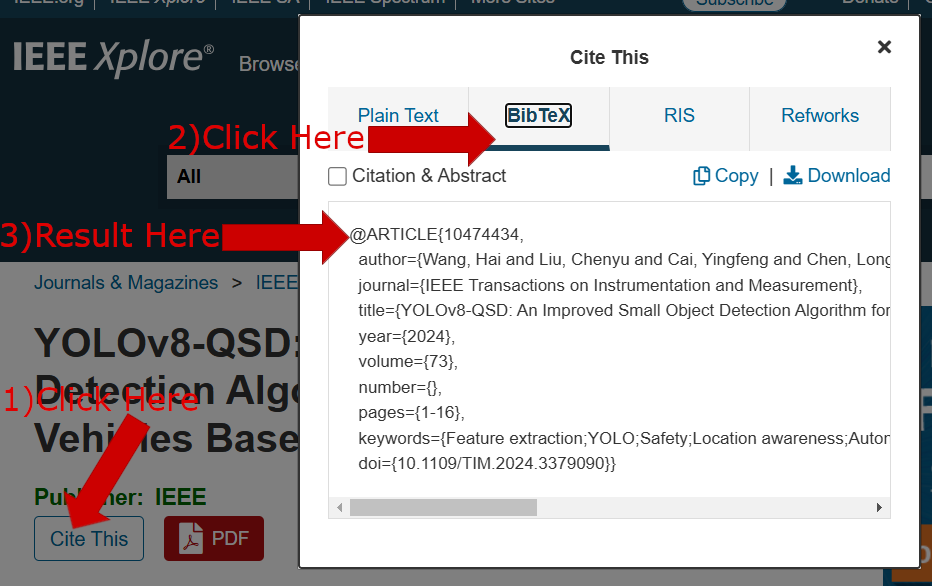
\includegraphics[width=0.3\linewidth]{fig/IEEE-cite-step.png}} \hfil
    \subfloat[於Sciencedirect網站平台]{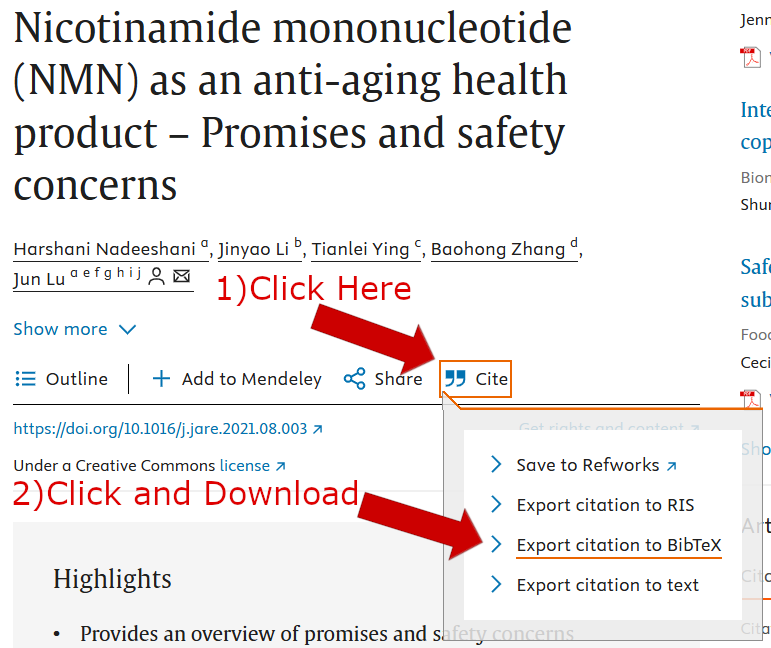
\includegraphics[width=0.3\linewidth]{fig/sciencedirect-cite-step.png}} \hfil
    \subfloat[於arXiv平台]{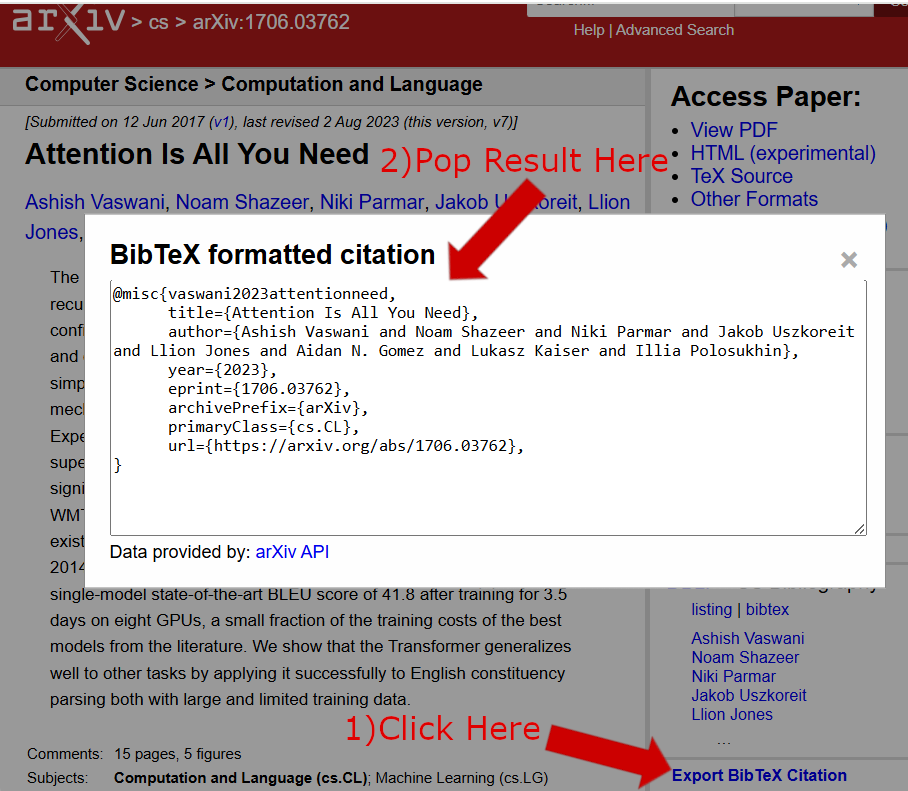
\includegraphics[width=0.3\linewidth]{fig/arxiv-cite-step.png}}
    \caption{不同平台\BibTeX 引用文獻格式取得步驟}
    \label{fig:citebibtex}
\end{figure}

\begin{figure}
    \centering
    \subfloat[使用Google Scholar生成]{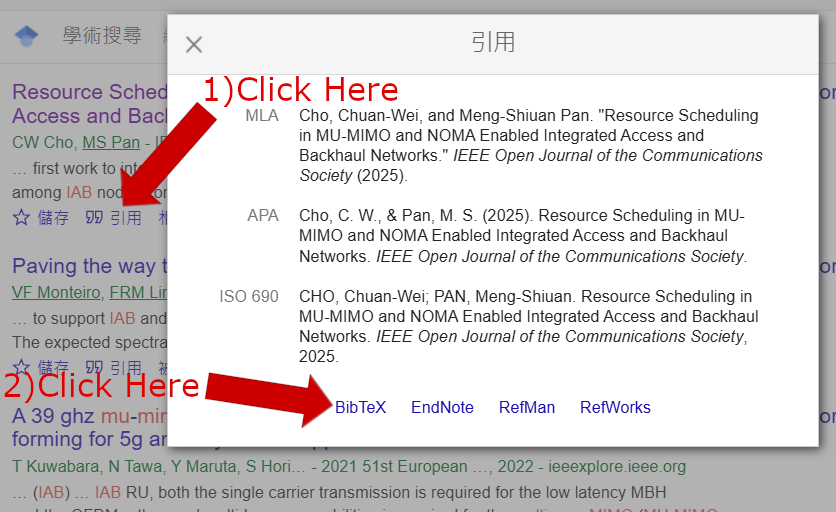
\includegraphics[width=0.4\linewidth]{fig/gcite-step.png}} \hfil
    \subfloat[生成的結果與推薦的引用名稱]{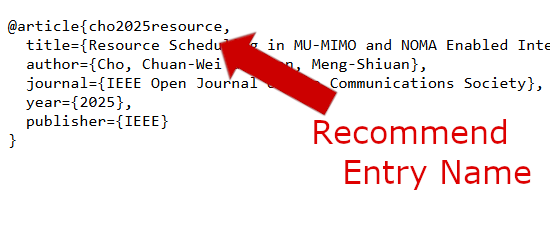
\includegraphics[width=0.4\linewidth]{fig/gcite-res-name.png}}
    \caption{使用Google Scholar生成\BibTeX 以及推薦的引用名稱}
    \label{fig:gscite}
\end{figure}

在圖\ref{fig:citebibtex}中使用紅色箭頭與對應的文字說明了
\begin{enumerate*}
    \item IEEE Xplore\footnote{即IEEE的線上數位資料庫平台,也就是平常IEEE論文的發布網站。}、
    \item Sciencedirect 網站與
    \item arXiv 網站產生\BibTeX 引用文獻格式的具體流程。
\end{enumerate*}
其中IEEE Xplore與arXiv會在點擊Cite This或Export BibTeX Citation後彈出一個網頁內的子窗口。IEEE Xplore需要再點擊 BibTeX 分頁才能找到結果,而arXiv的窗口內則直接是生成結果。Sciencedirect 網站則不太一樣,其點按Cite後可以生成多種格式的結果其中便有BibTeX選項,不一樣的是他會直將生成的結果作為指定檔案格式(如\code{.bib})下載而非在網頁上開啟。其他平台雖然沒有提及,但是多半也能在``\textbf{Cite}''或``\textbf{Citation}''等關鍵字上找到對應的引用格式生成功能。如果無法方便的找到官方的生成結果也可以使用 Google Scholar 自動生成的 \BibTeX ,其具體過程可以參考圖\ref{fig:gscite}。簡而言之,Google Scholar上可以直接在搜尋條目下方找到``引用'',點擊後一樣會產生一個網頁內的子窗口其中有個``\textbf{BibTeX}''連結,點按之後可以得到類似於圖\ref{fig:gscite}(b)的\BibTeX 結果。

值得注意的是,由於我們希望在\LaTeX 撰寫過程中還是希望能足夠方便且簡短的區分文獻,因此時常會建議使用``年分''、``作者姓''與``文章標題單詞''取代圖\ref{fig:citebibtex}(a)中那樣流水編號或者\ref{fig:citebibtex}(c)那樣過長的名稱。這時可以注意到圖\ref{fig:gscite}(b)中 Google Scholar自動生成的 \BibTeX 其引用名稱剛好符合合適的命名需求。因此,個人建議\BibTeX 文獻命名可以直接使用 Google Scholar 所生成的結果\footnote{具體的\BibTeX 內容還是以官方提供的訊息為準進行調整更不容易出錯。}。另一方面,通常而言\LaTeX 排版時會傾向於將``title''參數的內容以僅首字母大寫的方式排版,這時標題有些必須大寫的部分會被錯誤排版。同樣以\cite{ieeebib}舉例,在上面給出的代碼中``title''部分在最終排版結果中會變得非常難看 (因為本文中也沒有為其進行特別調整),實際上在要求參考文獻排版時我們應該把那些需要維持大小寫的部分以\{...\}的方式包起來,以做出類似於如下的改進
\begin{lstlisting}
@misc{ieeebibAlt,
  title        = {How to Use the {IEEEtran} {BibTeX} Style},
  author       = {Michael Shell},
  year         = {Feb. 2025},
  note         = {\url{https://tw.mirrors.cicku.me/ctan/macros/latex/contrib/IEEEtran/bibtex/IEEEtran_bst_HOWTO.pdf}},
  howpublished = {IEEE}
}
\end{lstlisting}
這時如\cite{ieeebibAlt}的結果便會是符合我們預期、較為美觀且正確的排版方式。

至此,\BibTeX 文獻格式的主要使用方式已經大致上介紹完畢,而整體上本模板與\LaTeX 的基本使用方式也已經完成說明。然而\LaTeX 是一個圖靈完備的排版語言,在實際使用過程中可能仍會遭遇到一些排版的問題與需求需要使用更多的Package、經驗\footnote{由於\LaTeX 作為沒有命名空間,甚至於語法邏輯都是基於巨集(Macro)的古老程式語言,指令的順序、Package順序等等都有可能影響代碼執行的具體行為。}甚至複雜的代碼解決,甚至有些問題對於不熟悉排版術語的使用者來說可能難以準確地描述足以搜尋的提問。好在,僅考慮學術與學位論文寫作中所會遭遇的問題都較為單純而且提問的人較多,在接下的來的章節中我們會進一步說明一些常見的學位論文排版問題。此外,這裡也會為初次撰寫論文的圖者提供(學位)論文的基本撰寫思路。

\chapter{常見問題}

許多初入\LaTeX 的使用者也是第一次作為研究生至撰寫具備學術性質或者說論文性質的文章。這時會有很多人不知所措,不知道從何起頭,也不知道如何收尾,更可能會疑惑「做好」為何如此困難。簡而言之,正是因為「第一次」的身份,``我們''沒有一個適合的評斷依據與參考標準去判斷自己的決策與自己所撰寫的文章是否是導師們想要的亦或者是否是自己所想要的。這些問題在大語言模型當道的現在很多都已經不再是問題,但是缺乏經驗的``我們''也仍需要依據與思路去判斷AI所描述的是否正確,而我們又應當如何使之更加符合我們的需求。這一章節會簡要地解釋與描述一些常見的問題,以使得這份模板可以不僅僅作為代碼意義上的``模板'',也能為有需要的使用者提供一些必要的思路。

\section{文章結構}

\subsection{入門寫作指引}

萬事起頭難,對於大部分的研究生而言「如何為自己的論文開頭?」又「如何安排自己的文章架構」通常是最艱難而苦澀的時候。尤其是當我們並不知道「為什麼」要這麼做的時候。而這一切「為什麼」實際上問題在閱讀其他已發表的學術期刊論文時就已經開始醞釀。

如何讀懂一篇論文是需要大量練習與訓練。這裡所練習與訓練的並不是如何在\textit{\textbf{語言}}的層面看懂一篇論文,而是在\textbf{\textit{需求}}與\textit{\textbf{目標}}的層面看懂一篇論文。論文這個格式作為當前學術研究的主流載體,雖然在日新月異的數位時代其版面與格式或許已經有些過時與落伍,但是其文章結構仍有其值得參考的意義。雖然期刊論文與學位論文常用的文章結構略有不同,但是參考期刊論文常見的論述結構我們能更加直觀地明白論文這種載體想要的是什麼效果,而學位論文又是因為什麼原因而有了微妙的不同。

以個人認為中文的「論文」一詞是相當優雅且準確的稱呼,比起paper, article, report, essay, $\dots$ 等等英語上的細分規格都更能體現這種文字體裁所應具備的含義。依我之見,論文的意義在於論述觀點,而如何系統性地展示「這個觀點」的價值與意義正是「論文」的文章結構上應該具備的能力。我們可以注意到,常見的論文體裁通常文章結構都不會缺少下面幾個部分
\begin{enumerate}
    \item 緒論/介紹 (Introduction)
    \item 相關文獻 (Related Works)
    \item 系統模型 (System Model)
    \item 問題定義 (Problem Definition)
    \item 提出方法 (Proposed Method)
    \item 模擬/實驗結果 (Simulation/Numerical/Experiment Results)
    \item 總結 (Conclusion)
\end{enumerate}
這樣的文章結構只是「模板」亦或者這有其原理,很多人都有自己的看法。而我希望回歸到我一開始的表述「論文是一種用以表達觀點,並說明觀點意義的文章體裁」。這個表述其實本身伴隨著一個問題,即「我們要如何\textbf{\textit{說明}}和\textbf{\textit{證明}}這個觀點的意義呢?」這個問題的答案便是其結果。

「很多時候,問題遠比答案更重要。」如果一個觀點有意義,就意味著這個觀點經的起各種方面的質詢(提問)。首先,如果要能說服一個人某個觀點是具有意義的,那麽這個觀點必須對於現實世界或是邏輯思維上具備指導性。我們無法說明一個「憑空出現」且難以定義的事物或問題是否具有意義,因此我們需要讓我們的觀點與現實世界或是與某種現今已知的邏輯概念發生交集(即便只是數學意義上)。為了說明一個觀點與現有事物/概念的連結,並指出這個觀點並非憑空而生而是有著清晰的邏輯脈絡 (動機),因此我們會需要一個章節(緒論/介紹, Introduction)去說明這一切。

接著,也同樣由於一切並不會憑空發生,我們需要有現今已知、已被認可的事物為我們的觀點背書。此外,沒有人喜歡重複造輪胎。一個已經被人所研究過、論述過的觀點,不需要再沒有理由、沒有觀察的重新研究一次。如果我們的觀點是新的,就意味著過往的觀點必須是舊的;如果我們有新觀察是對的,那就意味著過往的觀察是錯的或是需要補充的。而我們要如何證明這點,便只能舉證足夠數量或者足夠有代表性的過往觀點。這不僅是一種演辯工具,讓過去的研究,也成為支持你觀點的武器;也是在巨人的肩膀上,讓過去的堆砌,推砌成足以見證全新風景的台階。這便是需要過往``相關文獻 (Related Works)''的理由。

我並沒有打算每一章節的概念都以上述的形式說下去,我們必須真正直指那問題的核心----「很多時候,問題遠比答案更重要」。觀點與問題往往相映而生,「如果多了這個考量$\dots$?」這時考量便成了某些「變化」形成的觀點,而在提出「為什麼這個現象在$\dots$會發生?」爾後問題本身孕育著即將孵化的答案 (觀點)。我們需要足夠清晰的去\textbf{\textit{描述}}我們的問題從而引導我們的\textbf{\textit{觀點}}得以在他人的思想中孵化。系統模型與問題定義常常出現在同一個章節之中,正因為他們本來就為了這樣相同的目的而生。

「你說的很對,那我問你,你怎麼能證明你的方法的正確性呢?」---證明,就是論述我們觀點意義的最後一步。我們可以有很多種方法,而實驗與模擬往往是最直白的。基於一個簡單的邏輯,在環境本身不變的情況下,基於我們觀點產生的方法去與過往不包含我們觀點的方法比較,觀察是否在我們所設想的具體指標上存在如我們所述的影響,這便是提出方法與模擬實現的意義。而在這之後理所當然的,重新描述自己的觀點與驗證流程,為我們的觀點論述作出總結。

很多人說,寫論文就像是寫故事。我想這並沒有錯。論文是給人閱讀的,我們需要讓人能讀下去、能理解最終才能明白我們所希望他們知道的。「摘要」是一個給自己論述的這個故事一個貼合文章結構而且吸引人的介紹,讓人可以一眼就看出來你的觀點哪裡吸引人而又哪裡與眾不同。

最後,我們回到一個問屜「學位論文」到底微妙的差在哪裡呢?依我之見,學位論文不僅僅只是一個闡述觀點的「論文」,它還具備了兩項功能
\begin{enumerate*}
    \item 作為教育單位學術研究的總結性結果,其還可以是對後輩新人的指引,以及
    \item 作為畢業條件其同時也是對於自身專業理解、專業能力的側寫。
\end{enumerate*}
因此許多的學位論文不僅僅是觀點的呈現,同時也兼具著許多科普的責任,需要明確的展示自身對於這些專業領域的概念有著足夠的理解,也需要能證明自己的理解足以引領他人入門。

\subsection{其他常見文本排版問題}

上面介紹了論文寫作的大致要點,接下來對於論文文本本身排版有些要求,特別是在意中英文混合排版的讀者可以特別注意一些問題。特別是理工類的中文論文無法避免中英文混合排版的問題,這裡對於中英文混合排版有幾個簡單的建議。
\begin{enumerate}
    \item 專有名詞與專業術語至少在文章中首次出現時應列出其英文名稱,而這個詞彙如果會在文章中大量出現通常會順便舉出其縮寫。舉例而言,低地球軌道 (Low Earth orbit, LEO) 衛星、基地台 (Base station, BS)、積體電路 (Integrated circuit, IC)。如果不確定一個名詞是否應該舉出英文名稱,就應該列出英文名稱,因為這意味著該詞彙本身就並不足夠大眾(為人所知)。
    \item 在全文中風格與用詞統一。由於一個名詞概念同時有英文、中文和縮寫三種表達形式,在文章中除了名詞第一次出現以外其餘時候盡可能只使用唯一一種表達形式以保證文章閱讀順暢。而英文詞彙上是首字母是否大寫主要也是以閱讀舒服美觀為主。如果是常見的名詞且不在句首則全文統一風格即可,如果是專有名詞或有特別意義的詞彙則建議首字母大寫,而如果是標題則建議除了介系詞之外各個單詞首字母都大寫。
    \item 確保中英文用詞無歧義。不論是在中文或者英文中,有許多詞彙需要特定上下文才能明確其無歧義的含義。因此,有些詞彙在使用前應該在搜尋階段確保含義正確以避免誤用,或者藉由中英文對照明確其所表達的含義。其中最常出現的誤用是標準化、正規化這類習慣用詞,不僅計算過程應在文章中將其明確定義,也需要在資料搜集階段就確定應該是Standardize, Normalize 或者甚至於 Maximum absolute scaling。合理且明確的用詞可以增加自己的專業度,也能顯著的提升文章的易讀性。
    \item 中英混合排版時有時候英文與中文之間應有的間距(空白)會遺失。如果要避免這項狀況發生 English Text 和中文文字之間可以在撰寫文章時主動留白。除此之外,英文字詞與括號在\LaTeX 中不會主動產生空白(間距),因此當使用當英文單字與括號相鄰時需要主動的留出空白以避免極其難看的排版。這種狀況常見於縮寫的使用上,舉例而言我們更希望看到 ``Table of Contents (ToC)'' 而不是 ``Table of Contents(ToC)''。
\end{enumerate}

\section{符號系統設計}

很多人在撰寫學位論文時才第一次接觸到使用數學語言的形式描述問題,這時不要懷疑,和寫程式不一樣的在論文的形式上符號精簡而優美而易於理解才是正道。我們已經在文章種解釋過一次符號的意義了,我們就不需要再為符號取冗長的名稱了。為了方便理解與,通常這符號會參考下英文翻譯,像是容量的``capacity''可以用$c$表示,如果太多不同的\textit{capacity}我們還有上下標、大小寫、\showcmd{hat\{c\}}、\showcmd{bar\{c\}}甚至$c'$可以使用。

也還要記得,數學上本來就有一些常用的符號,像是代表函數的$f$/$F$, $g$/$G$, $h$/$H$,或是常用來作為索引的$i$,$j$,$k$,以及常常作為標變數的$a$,$b$,$x$,$y$,$z$,以及常見的那些$\alpha$, $\beta$, $\gamma$,這些符號都時常用作抽象概念的代表符號使用。更重要的是參考已經看過的論文,對於不同領域時常有一些常見的、大家熟悉的符號系統。有些甚至會取代原有的符號慣例,像是機器學習裡面的 $Q$, $\pi$, $\dots$,還有訊號處理裡常常直接使用$y$,$x$作為訊號,有些已經成為符號設計的「慣例」都可以記錄下來在論文中加以利用。

\section{美化排版}

研究生群體裡從來不缺少對於排版有美觀追求的人,但往常使用MS Word時由於排版與文字內容耦合度高,對於論文「排版」本身的美感追求反而會使文字內容編輯工作變得十分彆扭 (特別是雙欄排版格式下圖片與表格的位置調整)。但是在\LaTeX 上內容與排版的解耦,為一些排版上的美感追求挪出了空間。然而由於\LaTeX 本身語法的複雜性以及臃腫且過時的庫管理,實際上要做出美觀的排版對於新使用者而言並不友善也相當耗費時間與心力。因此,在這一節中介紹了一些較為常用且實用排版語法,為有一些美觀追求的使用者減少心神的消耗。

\subsection{多圖與跨欄排版}

對於多圖排版常見的有兩種方式,一種是如圖~\ref{fig:multifig1}使用表格進行多圖排版,另一種則是如圖~\ref{fig:multifig2}使用樣式包進行多圖排版。

\begin{figure}[t]
    \centering
    \begin{tabular}{ccc}
         
\includegraphics[width=0.3\linewidth]{fig/Gemini_Generated_Image_53joui53joui53jo.jpg}
         &
\includegraphics[width=0.3\linewidth]{fig/Gemini_Generated_Image_8hz5mu8hz5mu8hz5.jpg}
         &
\includegraphics[width=0.3\linewidth]{fig/Gemini_Generated_Image_k9qf9ik9qf9ik9qf.jpg} \\
         (a)&(b)  &(c) \\
    \end{tabular}
    \caption[使用表格的多圖排版演示]{由 Gemini 產生的圖片。(a) 藍色的純色圖片 (b) 橘色的純色圖片 (c) 適合與藍色和橘色搭配的顏色。}
    \label{fig:multifig1}
\end{figure}

\begin{figure*}
    \centering
    \subfloat[]{
        
\includegraphics[width=0.3\linewidth]{fig/Gemini_Generated_Image_53joui53joui53jo.jpg}
        \label{fig:1}
    }
    \subfloat[]{
        
\includegraphics[width=0.3\linewidth]{fig/Gemini_Generated_Image_8hz5mu8hz5mu8hz5.jpg}
        \label{fig:2}
    }
    \subfloat[]{
        
\includegraphics[width=0.3\linewidth]{fig/Gemini_Generated_Image_k9qf9ik9qf9ik9qf.jpg}
        \label{fig:3}
    }
    
    \caption[使用\showcmd{subfloat}的多圖排版跨欄演示]{由 Gemini 產生的圖片。(a) 藍色的純色圖片 (b) 橘色的純色圖片 (c) 適合與藍色和橘色搭配的顏色。}
    \label{fig:multifig2}
\end{figure*}

有些論文排版格式會要求雙欄,這時多圖排版容易侵犯到另一欄導致排版出現問題。在\LaTeX 中對於浮動環境提供了跨欄的排版,只需要將原先的環境名稱後加上\code{*}即可。具體而言,一般的浮動圖片排版如下
\begin{lstlisting}
\begin{figure}
....
\end{figure}
\end{lstlisting}
而跨欄的浮動圖片排版則如下
\begin{lstlisting}
\begin{figure*}
....
\end{figure*}
\end{lstlisting}
除了跨欄的圖片排版之外,跨欄的表格排版也常被使用,這裡也直接提供具體的環境名稱\code{table*}。

\subsection{簡化引用}

至此應該有人注意到\code{\showcmd{ref}}指令只會生成標號,如果需要``圖. n''這樣的常用結構就需要一直輸入\code{圖.\showcmd{ref}}這樣的代碼結構。針對這樣的問題,我們可以自行定義指令如下
\begin{lstlisting}
\newcommand{\Fig}[1]{Fig.~\ref{#1}}
\end{lstlisting}
這樣我們便可以使用\code{\showcmd{Fig\{fig:multifig2\}}}這樣的代碼形式生成 \code{\Fig{fig:multifig2}}這樣的結果。在\code{macros\_clean.tex}中定義了一系列這樣的指令,如果需要可以自行於檔案中修改生成結果的格式,其中比較常用的指令包含如下
\begin{lstlisting}
\newcommand{\Eq}[1]{Eq.~(\ref{#1})}
\newcommand{\Fig}[1]{Fig.~\ref{#1}}
\newcommand{\Tab}[1]{Table~\ref{#1}}
\newcommand{\Algo}[1]{Algorithm~\ref{#1}}
\end{lstlisting}
其中我們額外建議,如果不習慣預設的\code{\showcmd{Algo}},可以將其修改為\code{\showcmd{Alg}}或者使用類似於下面的代碼在不修改原始定義的情況下新增指令
\begin{lstlisting}
\newcommand{\Alg}[1]{\Algo{#1}}
\end{lstlisting}

\subsection{標題斷行}

這是專屬於本模板的特有問題,自動化處理固然方便但是卻較難調整一些客製化的需求。有些人可能會注意到,有些標題在標題頁與封面頁斷行/換行之處並不好看。一般而言\LaTeX 上可以自行在標題中使用\code{\textbackslash\textbackslash}換行,但是在此模板中由於使用\code{\showcmd{settitles}}指令或者藉由\code{\showcmd{renewcommand}}修改\code{\showcmd{titlezh}}或\code{\showcmd{titleen}}的標題會被自動填入到多個地方,因此不能直接在這些指令中調整標題。

為針對這個問題,本文中額外定義了\code{\showcmd{setbigtitles}}、\code{\showcmd{setbigtitleszh}}和\code{\showcmd{setbigtitlesen}}指令可以單獨修改封面頁與標題頁的標題,具體而言我們可以如下使用這些指令
\begin{lstlisting}
\setbigtitleszh{中文\\標題}
\setbigtitlesen{English\\Title}
\setbigtitles{中文\\標題}{English\\Title}
\end{lstlisting}
需要特別\textbf{\textit{注意}}的是,這三個指令都需要在原先標題指令使用之後、封面頁生成指令使用之前使用才能正常生效。

\subsection{表格}

有注意到的人應該有注意到了,在上面的演示中\LaTeX 中的表格使用\code{c}, \code{l}, \code{r}表示表格直欄的文字對齊方式為置中、靠左或靠右。而這三個指令都會「自動改變表格寬度」,因此如果當文字過長時表格排版就會超出合理的版面範圍。在演示中同樣也呈現了使用\code{p}指令限制表格大小的方法,但是這個方法默認情況下只會靠左對齊。如果需要在\code{p}模式下使用其他對齊方式可以參考\cite{latextabp}並可以使用\cite{latexntab}的方式簡化指令。

在表格中另一個常用功能是合併行或列,在\LaTeX 中這是一項複雜的功能,具體語法可以參考官方文檔\cite{latextabmul}中``\textbf{Combining rows and columns}''小節。而複雜的複合合併則可以參考\cite{latextabcomplex},主要細節是行列的合併嵌套有一定順序,否則有可能會出現編譯錯誤,一般而言嵌套方式如下
\begin{lstlisting}
\multicolumn{2}{c|}{\multirow{2}{*}{Multi-Row and Col}}
\end{lstlisting}

\subsection{美化公式}

先前演示過一些常用的數學公式語法,但是卻沒有介紹過數學公式的排版。數學公式的排版也是由「環境」構成並且與表格十分相像但又更加複雜,首先目前最為推薦使用的是\code{split}環境。這個環境只做簡單的「單錨點」排版。具體而言可以參考下面方程
\begin{equation}
    \begin{split}
        y &= \frac{1}{3}\times \frac{4}{9} \times \frac{36}{16}\\
          &= \frac{1}{3}\times \frac{4}{9} \times \frac{9}{4}\\
          &= \frac{1}{3}\\
    \text{Ans:}&\ \frac{1}{3}
    \end{split}
\end{equation}
在這個環境中 $\&$ 是錨點,所有公式的排版會以 $\&$ 對齊,並以換行符號換行。這種排版簡單、實用、常用,而且可以較為易於理解的與其他環境一同使用,如
\begin{equation}
    \begin{split}
        f(x) =& \\
    &\begin{cases}
        f(x-1)+1, &x=\mathrm{cond},\\
        0, &x\neq \mathrm{cond}
    \end{cases}
    \end{split}
\end{equation}
另一種更為強大但是複雜的環境是\code{aligned},這個環境可以定義排版的「欄位」和「錨點」。具體而言,我們可以參考下面代碼
\begin{equation}
\begin{aligned}
    x=&1.1 & y=&1.2 & z=&1.3\\
    x1=&2.1 & y1=&2.2 & z1=&2.3 \\
    letft& & cen&ter & &right
\end{aligned}
\end{equation}
在這個排版環境中「奇數」的\code{\&}是該直欄的「錨點」,而「偶數」的\code{\&}則是和表格一樣的「分欄」符號。除\code{aligned}之外,\LaTeX 中還有\code{align}環境與\code{align*},只是這兩個環境是用來分別取代\code{equation}和\code{\showcmd{[}\showcmd{]}},而不像\code{aligned}是「數學環境」內的環境。而\code{align}與\code{align*}具體的區別也如上面所述,\code{align}有以「行」為單位的編號而\code{align*}沒有編號。

除此之外,這裡還必須介紹\code{\showcmd{left}}與\code{\showcmd{right}}指令。在上面的演示中應該有人注意到如果撰寫如下代碼
\[
(\frac{\log_m a}{\log_m b}) = \log_a b
\]
小括號\code{(...)}無法匹配其所應包裹的內容,這時的排版沒有錯誤但是難以說得上美觀。而\code{\showcmd{left}}與\code{\showcmd{right}}指令便是用來解決這樣的問題,這兩個指令總是成對出現、讀取該指令後一個用於``包圍''其他數學內容的字符\footnote{通常而言這個字符包含(,),[,],\{,\},|,$\|$等等。},並且可以將這些字符延展到足以包圍其內容的數學元素。使用這兩條指令我們可以重寫代碼如下
\[
\left(\frac{\log_m a}{\log_m b}\right) = \log_a b
\]
這兩個指令對於符號的匹配實際上相當自由,我們甚至可以寫出下面的符號排版
\begin{equation}
\left|
\begin{aligned}
    x=&1.1 & y=&1.2 & z=&1.3\\
    x1=&2.1 & y1=&2.2 & z1=&2.3\\
    letft& & cen&ter & &right
\end{aligned}
\right)
\end{equation}
如果我們只需要單邊的括號,我們可以用下面讓\code{\showcmd{left}}或\code{\showcmd{right}}讀取\code{.},藉此我們甚至可以使用\code{aligned}實現如同\code{cases}環境效果的代碼如
\begin{equation}
\mathrm{Eq(x,y)} = 
\left\{
\begin{aligned}
    &1, &x=y\\
    &0, &x\neq y
\end{aligned}
\right.
\end{equation}
至此,如何美化與自定義數學模式下的``排版''的方法大致上都已經介紹完畢。實際上美觀的數學定義仍有許多排版以外的要素存在,包含字體、符號使用、上下標等等。但是這些美觀的需求往往都需要更多的經驗取得而非三言兩語所能知之。如果不知道如何展示美觀的數學表示,至少需要謹記
\begin{enumerate*}
    \item 盡可能的簡潔而且清晰、
    \item 上下標邏輯意義明確且統一、
    \item 一個公式僅表達一個概念 (或觀點)。
\end{enumerate*}
此外,若無必要勿使用長單詞,如有必要則使用\showcmd{mathrm}調整常單詞字體增加可讀性。一般而言讀者更希望看到$\mathrm{SINR}$而不是$SINR$或$sinr$,以$SINR$而言排版上會更像多個各自具備意義的符號,而$sinr$則本身並不易於閱讀。因此我們更希望使用\showcmd{mathrm\{\}}將應該被視為單詞排版的詞彙在數學模式下依然作為單詞(通常是函數)進行排版,從而提升可讀性並更加美觀。

\subsection{程式代碼}

代碼環境就不過多贅述,上面的文本中已經使用過非常多次了,在這裡僅提供一些合適的文獻參考,如Overleaf官方文檔 \cite{latexlstoverleaf} 和 wikibooks \cite{latexlstwiki}。如果要說特別需要注意的地方,我建議使用\code{\showcmd{lstset}}設定全局的樣式 (本範中該設定於\code{style.tex}),並在局部使用\code{[...]}定義樣式,如:
\begin{lstlisting}[language=Python]
def main() :
    print('Hello, world!')
if __name__ == '__main__' :
    main()
\end{lstlisting}
若是需要C語言語法樣式則能改為\code{[language=C]]}
\begin{lstlisting}[language=C]
#include<stdio.h>
int main (void){
    printf("Hello, world!\n");
    return 0;
}
\end{lstlisting}

\subsection{函數定義與演算法}

有些人可能會需要在演算法裡面定義函數,在具體方法上面實際上有相當多種。這裡僅舉例一個最最簡單的方式,即「實際上演算法環境也只是一種特殊的浮動表格」所以我們可以單純的「描述」函數,在很多的字排版軟體中是用這種方法操作。其中一種方法參考至\cite{latexfunc},其具體範例可以參考如下

\begin{algorithm}
\caption{一個清楚的演算法標題}
\label{alg:func}
\SetKwFunction{FuncVar}{FunctionName}
\SetKwProg{FuncCmd}{Function}{:}{}
\FuncCmd{\FuncVar{$args$}}{
something\;
}
\end{algorithm}

\section{參考文獻格式}

對於理工系學生來說,IEEE格式幾乎可以被視為標準的參考文獻格式,這時我們可以直接使用\code{\showcmd{bibliographystyle\{IEEEtran\}}}定義我們的參考文獻格式是符合IEEE的格式。但是\code{IEEEtran}格式多定義了一些格式上的描述,因此如果我們需要一些非其規定的特殊格式時可能無法簡單的修改而成。為滿足遇到特殊格式時的需求,這裡我們稍微討論一下如何「排出」參考文獻格式。

\subsection{引用網頁}

舉例而言,如果我們當前只有\code{ieeetr}格式,想要排出\code{IEEEtran}中網頁的排版效果。我們可以先參考BibTeX官網 \cite{bibtex} 中對於\code{misc}或這其他類型格式的介紹,再比較其與IEEE規範\cite{ieeebib,ieeerefguide}之間的區別,直接用文字的方式「拼出」需要的格式。舉例而言,本模板\code{ref.bib}中BibTeX官網 \cite{bibtex}的BibTeX 格式文獻條目如下
\begin{lstlisting}
@misc{bibtex,
  title        = {The 14 BibTeX entry types},
  author       = {Paperpile LLC},
  year         = {Feb. 2025},
  url          = {https://www.bibtex.com/e/entry-types/},
  howpublished = {}
}
\end{lstlisting}
這個目錄在\code{IEEETran}格式下可以直接編譯出符合IEEE規範的網頁參考文獻格式
\begin{mdframed}
P. LLC, “The 14 bibtex entry types,” Feb. 2025. [Online]. Available: \url{https://www.bibtex.com/e/entry-types/}
\end{mdframed}
可是當使用\code{ieeetr}時會編譯出如下明顯不符合規範的格式
\begin{mdframed}
P. LLC, “The 14 bibtex entry types,” Feb. 2025.
\end{mdframed}
如果我們真的需要用\code{ieeetr}或是其他風格生成符合格式的參考文獻可以參考類似於 \cite{bibtexAlt} 的所定義的BibTeX如下
\begin{lstlisting}
@misc{bibtexAlt,
  title        = {The 14 BibTeX entry types},
  author       = {Paperpile LLC},
  year         = {Accessed: Feb. 2025},
  note         = {[Online.] Available: \url{https://www.bibtex.com/e/entry-types/}},
  howpublished = {}
}
\end{lstlisting}
具體而言,我們手動加入了``\textit{Accessed:}''和``\textit{[Online.] Available:}''等格式中所規範的描述方式。使之經由BibTeX編譯排列之後可以生成合理的參考文獻格式。其他不同類型的參考文獻格式在沒有可用的預定義風格(格式)時,也可以用相似的手法生成正確的參考文獻格式。

\subsection{引用arXiv}

另一個常見的引用來源是arXiv網站 \cite{arxiv},這是許多重要的開源文獻以及論文預印本所使用的發表平台,其主要內容包含數學、物理、工程與人工智能。特別是對於人工智能領域,該領域中許多重要的研究結果包括但不限於YOLO \cite{redmon2016lookonceunifiedrealtime}和Transformer\cite{vaswani2023attentionneed}都發表於該平台。然而作為純電子出版的開源平台,其合理的引用格式便成為了一項有待議論的問題。

如上面兩篇文章 \cite{redmon2016lookonceunifiedrealtime}, \cite{vaswani2023attentionneed} 在arXiv平台上所提供的BibTeX是以網頁的形式引用,但是若參考一些主流期刊的引用格式\cite{wang2024yolov8}則並非如此。在此,我們也基於Google Scholar所提供的BibTeX模板提供arXiv文獻引用格式的``拼湊''方式。首先,先注意到\cite{wang2024yolov8}中對於一篇arXiv文章\cite{ge2021yolox}的參考排版結果為
\begin{mdframed}
Z. Ge, S. Liu, F. Wang, Z. Li, and J. Sun, “YOLOx: Exceeding YOLO series in 2021,” 2021, \textit{arXiv:2107.08430}.
\end{mdframed}
這個格式顯然不是網頁格式 (由arXiv平台自動生成) 的引用。而現在此引用\cite{ge2021yolox}使用的是Google Scholar所生成的BibTeX
\begin{lstlisting}
@article{ge2021yolox,
  title={Yolox: Exceeding yolo series in 2021},
  author={Ge, Zheng and Liu, Songtao and Wang, Feng and Li, Zeming and Sun, Jian},
  journal={arXiv preprint arXiv:2107.08430},
  year={2021}
}
\end{lstlisting}
其排版的生成結果為
\begin{mdframed}
Z. Ge, S. Liu, F. Wang, Z. Li, and J. Sun, “Yolox: Exceeding yolo series in 2021,” \textit{arXiv preprint arXiv:2107.08430}, 2021.
\end{mdframed}
我們可以注意到,這兩者之間的排版差異並不是多一些字,而是排版順序也不一樣。此時可以參考IEEE文檔 \cite{ieeerefguide} 中對引用arXiv文獻的格式説明,再參考 \cite{ieeebib}, \cite{bibtex}, \cite{bibtexsty} 調整輸入參數,於是我們可以得到下面的BibTeX
\begin{lstlisting}
@unpublished{ge2021yoloxAlt,
  title        = {{YOLO}x: Exceeding {YOLO} series in 2021},
  author       = {Ge, Zheng and Liu, Songtao and Wang, Feng and Li, Zeming and Sun, Jian},
  year         = {2021},
  note         = {{\itshape arXiv:2107.08430}}
}
\end{lstlisting}
其中由於原先的\code{note}沒有斜體效果,因此這裡使用了\code{\showcmd{itshape}}指令用於生成斜體字體並藉由\code{\{\itshape ...\}}不讓其效果外溢到其他項目,這個BibTeX的排版結果可以參考\cite{ge2021yoloxAlt}
\begin{mdframed}
Z. Ge, S. Liu, F. Wang, Z. Li, and J. Sun, “YOLOx: Exceeding YOLO series in 2021,” 2021, \textit{arXiv:2107.08430}.
\end{mdframed}
此時的排版格式便已經與IEEE期刊\cite{wang2024yolov8}與IEEE規範\cite{ieeerefguide}, \cite{ieeebib}完全一致。其他需要的參考文獻格式也可以用相似的方式藉由這些參考資料\cite{ieeerefguide}, \cite{ieeebib}, \cite{bibtex}, \cite{bibtexsty} 產生。

\chapter{北科口試與離校作業細節}

雖然北科已經在教務處頁面 \cite{ntutfinal} 提供了口試、畢業與離校相關的資訊,但是細節流程上的資訊零散的分散在教務處和圖書館的各個介面上。在這個章節中,我會根據自身的經驗整理從口試到離校的細節流程、所需的文件以及一些注意事項 \textit{(以下流程皆以電子工程系為例)}。

\section{口試前準備}

口試前的準備工作除了\cite{ntutfinal}以外還需主要參考三個網頁的內容,其中包含
\begin{enumerate*}
    \item \linkurl{https://oaa.ntut.edu.tw/p/412-1008-12839.php?Lang=zh-tw}{表單下載} \cite{ntutsheet}、
    \item \linkurl{https://lib.ntut.edu.tw/sp.asp?xdurl=mp100/SLP.asp&ctNode=1604&CtUnit=460&BaseDSD=7&mp=100}{圖書館畢業生專區} \cite{ntutlibgraduate} 以及
    \item \linkurl{https://cloud.ncl.edu.tw/ntut/}{碩博士論文系統 (國圖)} \cite{ntutlibupdate}。
\end{enumerate*}
這三個網頁實際上只為解決\textbf{口試申請}以及\textbf{論文查重}\footnote{重複率審核}這兩件事情。我在這裡整理了詳細的細節,方便畢業生作業的進行。

\subsection{口試申請}

首先,這個階段在\linkurl{https://oaa.ntut.edu.tw/p/412-1008-12839.php?Lang=zh-tw}{表單下載} \cite{ntutsheet} 頁面的 \textbf{(J) 學位考試區}中需要四份表單,其中包含
\begin{itemize}
    \item \textbf{學位考試申請書}:碩士班和博士班分別是 (J1) 和 (J7)。
    \item \textbf{學位考試\ 委員名單}:碩士班和博士班分別是 (J5) 和 (J8)。
    \item \textbf{學位考試申請名單彙整表-系所使用}:皆為 (J6)
    \item \textbf{國立臺北科技大學學位論文原創性比對檢核表\textcolor{red}{(口試版)}}:皆為 (J16)
\end{itemize}
\textbf{學位考試申請書}主要是為檢核是否已經完成碩士與博士在學制上的基礎目標,即檢核是否滿足\textbf{學分數}、\textbf{英文門檻}和\textbf{學術倫理測驗}等 (博士生還需完成\textbf{資格考}、\textbf{博士候選人}審核與\textbf{論文計點})。\textbf{學位考試\ 委員名單}是為檢核口試委員是否滿足學校所規定之資格,以北科而言沒有疑慮\footnote{一定符合規範}的口試委員為大學的\textbf{教授}與\textbf{副教授},但是需要注意\textbf{外校口委}的人數需求。口試委員盡可能及早邀請,以避免多個口試委員時間無法協調的狀況發生。如果口試委員發生變動則需要\textbf{學位考試委員異動申請表} (碩士為 (J2),博士為 (J10))。口試委員確認後,視各系規定可能還需要填寫\textbf{學位考試申請名單彙整表-系所使用}交給系所之承辦人員。\textbf{國立臺北科技大學學位論文原創性比對檢核表{(口試版)}}則需要配合圖書館方面的\textbf{論文查重}進行。這份表單有分為\textbf{口試版}與\textbf{定稿版},務必不要用錯。\textbf{學位考試申請書}、\textbf{學位考試\ 委員名單}都需要在\textbf{指導教授簽名}後送交至系辦公室 (或系所指定的其他單位),而\textbf{國立臺北科技大學學位論文原創性比對檢核表{(口試版)}}也需要簽名但是在口試完後繳交即可。簡略而言,如\cite{ntutfinal}所述在表單方面口試申請需要填寫並送出以下資料:
\begin{itemize}
    \item 學位考試申請書
    \item 論文初稿/摘要 (視系所規範)
    \item 歷年成績單
    \item 學位考試委員名單
    \item 學術倫理修業證明 (儘早在真正要口試之前完成)
    \item 英文門檻證明 (儘早在真正要口試之前完成並送核)
\end{itemize}

\subsection{論文查重}

論文查重方面的流程在 \cite{ntutlibgraduate} 的 \linkurl{https://lib.ntut.edu.tw/sp.asp?xdurl=mp100/SLP.asp&ctNode=1604&CtUnit=460&BaseDSD=7&mp=100\#top1}{論文原創性比對及複核}在細節流程上已經描述相當清晰。總略地來說,北科這裡論文查重有使用到
\begin{enumerate*}
    \item Turnitin \cite{turnitin} 和
    \item 國家圖書館臺灣博碩士論文知識加值系統 \cite{ntutlibupdate} 這兩個查重平台。
\end{enumerate*}
其中 Turnitin 大概每半年 (每學期) 更新一次查重的資料庫,其會比對國內外主流的學術論文資料庫中所包含的文章。而國圖的查重則著重在比對博碩士論文知識加值系統內所收藏的文章 (即過往的碩博論)。需要特別注意的是,Turnitin 的帳號需要先在\linkurl{https://lib.ntut.edu.tw/sp.asp?xdurl=mp100/genform.asp&mp=100&CtNodeId=1558}{圖書館的頁面}\footnote{https://lib.ntut.edu.tw/sp.asp?xdurl=mp100/genform.asp\&mp=100\&CtNodeId=1558}上\textbf{申請}再經由\textbf{人工審核}後才能使用,但可以使用非學校的常用電子郵件信箱進行註冊;而北科學位論文系統 \cite{ntutlibupdate} 的帳號則可以完全的\textbf{線上}註冊,但需要分為\textbf{兩個階段註冊兩個帳號}才能完成,細節可以參考北科的說明\cite{ntutlibupdate}的\textbf{帳號申請}說明。具體而言,其需要先註冊\linkurl{https://ndltd.ncl.edu.tw/}{博碩士論文知識加值系統}\cite{ndltd}的帳號,然後再用該帳號至\linkurl{https://cloud.ncl.edu.tw/ntut/in_pop3.php?school_id=316}{北科系統} \cite{ntut-ncl-reg} 註冊對應帳號。具體的論文比對操作可以參考\cite{ntutlibgraduate} \linkurl{https://lib.ntut.edu.tw/sp.asp?xdurl=mp100/SLP.asp&ctNode=1604&CtUnit=460&BaseDSD=7&mp=100\#top1}{論文原創性比對及複核}的\textbf{Step.2}中不同比對系統的\textbf{操作說明}。這兩個系統對於\textbf{即時的檢測}\footnote{大約5-15分鐘左右完成}都有\textbf{次數限制},其中國圖系統的即時檢測\textbf{總共}就三次,而 Turnitin 則是\textbf{每個上傳區塊 (不同作業標題)}都有3次的即時檢測機會。此外,這兩個系統都會顯示重複的文字段落以及重複來源,而 Turnitin 的系統還會呈現具體重複率 (百分比) 以及來源文章的相似文字片段。Turnitin 所標註的全部重複率和各個來源的重複率就是在\textbf{國立臺北科技大學學位論文原創性比對檢核表{(口試版)}}中要檢核的目標,原則上所有來源\textbf{合計}不能超過$20\%$,單一來源不能超過$2\%$。

當查重完成之後,正式口試前還需要完成\textbf{圖書館的複核}。這個複核需要在\linkurl{https://lib.ntut.edu.tw/sp.asp?xdurl=mp100/genform.asp&mp=100&CtNodeId=1600}{圖書館網頁上}\footnote{https://lib.ntut.edu.tw/sp.asp?xdurl=mp100/genform.asp\&mp=100\&CtNodeId=1600}進行申請,並由人工大概花費一個工作天左右完成。複核結果會以\textbf{電子郵件}形式回函,並且原則上在\textbf{口試時}需要\textbf{出示該複核結果}。在我自身的經驗中,這個複核過程更加傾向於確保``有正確的進行查重操作''\footnote{標題正確的同一初稿文章丟給兩個系統}而非看重於重複率本身。在申請複核時需要特別注意
\begin{enumerate*}
    \item 國圖的查重\textbf{報告}是否上傳到正確區塊 (作業標題)以及
    \item Turnitin\textbf{提交物件代碼}\footnote{申請的網頁上有連結指向足夠詳盡的說明頁面}是否填寫正確。
\end{enumerate*}

\section{口試中與口試完成}

在學位考試當天除了報告之外主要需要完成口試委員對多張表單的簽名與評分並送出考試委員的聘函 \cite{ntutlibgraduate}。這些表單同樣於 \cite{ntutsheet} 頁面的 \linkurl{https://oaa.ntut.edu.tw/p/412-1008-12839.php?Lang=zh-tw}{\textbf{(J) 學位考試區}} 下載,其中包含:
\begin{itemize}
    \item \textbf{學位考試-評分表} (J4):各個口試委員各一張
    \item \textbf{學位考試-成績表} (J15):一張
    \item \textbf{學位論文口試委員會審定書} (碩士 (J3), 博士 (J9))\footnote{或使用本模板提供的\LaTeX 編譯版}:一張
\end{itemize}
在口試完成之後需要向系辦繳回:
\begin{itemize}
    \item \textbf{學位考試-評分表}:委員簽名評分
    \item \textbf{學位考試-成績表}:委員(簽名)評分
    \item \textbf{學位論文口試委員會審定書}:委員簽名
    \item \textbf{學位論文原創性比對檢核表{(口試版)}}:指導教授與口試學生簽名
\end{itemize}

\section{離校過程}

根據口試結果修改完論文,並經由指導教授同意之後即可開始離校作業 \cite{ntutlibgraduate}。由於研究所學生被許可進行口試時基本上就已經確定除了畢業論文以外相關作業都已經完成了\footnote{口試申請的檢核內容},因此通常而言在電子論文的審核以外幾乎不會發生任何障礙。而為了進一步明確流程,減少些流程上可能發生問題,原則上的流程大致如下:
\begin{enumerate}
    \item 定稿版本論文上傳 Turnitin 審核,並下載報告書
    \item 定稿版本論文上傳國圖審核,並下載報告書
    \item 在\linkurl{https://oaa.ntut.edu.tw/p/412-1008-12839.php?Lang=zh-tw}{表單下載} \cite{ntutsheet} 頁面的 \textbf{(J) 學位考試區}中下載\textbf{國立臺北科技大學學位論文原創性比對檢核表(論文定稿版)} (J19) 並由指導教授與學生簽名
    \item 檢查電子論文格式 (套用本模板應該不會有問題,但編譯時仍須注意是有浮水印的書名頁開始)
    \item 在北科學位論文系統 \cite{ntutlibupdate} 中完成電子論文上傳並建檔。由於\LaTeX 原始內容即為無格式純文字,因此建檔過程大多數複製貼上原始文件中的內容即可。但是需要注意,英文人名為\textbf{姓氏在前}且全大寫的格式,如 ``王小明'' 應為 ``WANG, XIAO MING''。還要注意,\textbf{整個}論文的頁數以\textbf{阿拉伯數字}的為準。同時,在填寫目錄頁碼較為雜亂,需要注意是否填錯。
    \item 建檔完成後,印出兩份授權書 (注意標題,分別為北科圖書館和國家圖書館),並在指導教授與學生簽名後合併 (ZIP或單一 PDF)。
    \item 上傳合併後的授權書到學位論文系統
    \item 送出電子論文審核 (大約一到二個工作天)
    \item 完成審核之後編譯(或另外排版出)\textbf{紙本論文版檔案},並根據格式印刷紙本論文 (至少一本,更多則以系所和研究室規範為準),紙本論文\textbf{樣式}參考\linkurl{https://lib.ntut.edu.tw/sp.asp?xdurl=mp100/SLP.asp&ctNode=1604&CtUnit=460&BaseDSD=7&mp=100\#top6}{圖書館畢業生專區} 的 \textbf{6. 圖書館離校繳交} \cite{ntutlibgraduate}。
    \item 收到\textbf{審核完成的電子郵件}後印出電子郵件,並帶著\textbf{審核結果電子郵件}、\textbf{兩份授權書正本}與\textbf{紙本論文}送交至圖書館
    \item 至\textbf{入口網站}的\textbf{教務系統}中的\textbf{畢業生離校系統},根據內部步驟說明開始離校作業。
    \item 收到\textbf{離校審核完成}的電子郵件後,帶著印出的\textbf{審核通過電子郵件}與\textbf{學生證}至教務處領取畢業證書。
\end{enumerate}

\chapter{Conclusion}

這個範本本身是\schoolzh{}的學位論文格式範本,同時也是對於\LaTeX{}初學者與初次撰寫論文的研究者/研究生的引導文章。在本文中,一開始我們先介紹了如何使用這個範本,並且進一步說明了這個範本中所定義的一些自動化指令與環境。接著,我們藉由一篇短文介紹了\LaTeX{}的簡要使用說明,以自指形式排版並說明了\LaTeX{}撰寫論文時常用的指令。針對需要進一步瞭解如何使用\LaTeX{}美化排版,以及對於不知道學位論文應該如何起頭的讀者,這個範本中也使用了一個章節說明其中的細節並提供具體的引導。這篇總結也是一樣,期許為不知道如何文章撰寫讀者提供足以作為參考的指引。在本文中,除正文之外也存在一些為了「有趣」而使用的文案。雖然在實際的論文中這樣的文案並不合適,但是對於新生的使用者而言希望能理解---研究是嚴謹但是並不是嚴肅的事情。

\clearpage
\addcontentsline{toc}{chapter}{\bibname}
\bibliographystyle{IEEEtran}
\bibliography{ref}
\end{document}
